\documentclass[twoside]{report}
\usepackage[utf8]{inputenc}
\usepackage{graphicx}
\usepackage[a4paper,width=150mm,top=25mm,bottom=25mm,bindingoffset=6mm]{geometry}
\usepackage[english,spanish,activeacute,]{babel}
\usepackage[some]{background}
\usepackage{fancyhdr}

\backgroundsetup{scale=1,color=black,opacity=0.05,angle=0,contents={%
  
\includegraphics[width=0.5\paperwidth]{Documento_Latex/Imagenes/logo.png}}%
 }


\fancyfoot{}
\fancyfoot[LE,RO]{\thepage}
\pagenumbering{roman}

\title{Development of a Computational Desing Tool for Polypropylene-based composites having oxygen scavengers using the Hetereogenous Film Approach}
\author{Daniel Rozo}
\date{\Today}

\begin{document}
\begin{titlepage}
\begin{center}
\BgThispage
        \huge
        \textbf{Development of a Computational Desing Tool for Polypropylene-based composites having oxygen scavengers using the Hetereogenous Film Approach}
        
        \vspace{1cm}
        \LARGE

        \vspace{4cm}
        \textit{Author:}\\
        \textbf{Daniel Fernando Rozo Oviedo}\\
        \vspace{1.5cm}
        \textit{Supervisor:}\\
        \textbf{Felipe Salcedo Galan, PhD}
        \vfill
 
        First part of the thesis submitted for the degree of\\ Master in Chemical Engineering
        
 
        \vspace{1cm}
 
        
 
        \Large
        Deparment of Chemical Engineering\\
        Universidad de los Andes\\
        Bogotá, Colombia\\
        \today
 
    \end{center}
\afterpage{\null\newpage}


\end{titlepage}

\chapter*{Abstract}
\selectlanguage{spanish}
\begin{abstract}
\thispagestyle{plain}
\pagenumbering{roman} %
\setcounter{page}{3}
Uno de los principales tipos de empaques activos son los captadores de oxígeno (OS), los cuales son sustancias químicas cuyo propósito es reducir la cantidad de oxígeno residual en un paquete. Esto permite reducir el deterioro de los alimentos debido a la oxidación, prolongando así su vida útil. En el siguiente documento, el objetivo principal será desarrollar una herramienta computacional que permita el diseño de películas poliméricas captadoras de oxígeno. Actualmente, el grupo de materiales y manufactura CIPP-CIPEM de la Universidad de los Andes ha desarrollado películas de polipropileno que absorben oxígeno mediante la incorporación de aceite de linaza microencapsulado en sílice. En este caso, el aceite de linaza actúa como un agente absorbente de oxígeno activo. Para llevar a cabo la herramienta de diseño, surge la necesidad de desarrollar un modelo matemático que considere los detalles reactivos de la cinética de oxidación de la linaza, así como la distribución y evolución de los sitios activos dentro de la película polimérica. Con esto en mente, se desarrolló el enfoque de película reactiva y el modelo de película multicapa. Con el fin de implementar la naturaleza química de la oxidación del aceite de linaza, se realizó un ajuste sobre las constantes de velocidad cinética, así como sobre la concentración inicial de hidroperóxido y sustrato en el aceite. Los valores obtenidos logran predecir los perfiles de concentración experimentales, pero carecen de precisión para predecir los tiempos en que se desarrollan estos perfiles.
Con respecto a los métodos utilizados para resolver las ecuaciones del modelo matemático, se estudiaron varios algoritmos de diferencias finitas. Los resultados obtenidos al evaluar la precisión y el tiempo computacional mostraron que el mejor método para resolver el sistema de ecuaciones era el método de paso fraccional con una configuración de paso de tiempo adaptativo. Como conclusión principal de los resultados anteriores obtenidos, fue posible hacer una primera versión de la herramienta de diseño computacional. Esta versión es capaz de predecir la dinámica de los perfiles de reacción y concentración para películas absorbentes de oxígeno monocapa y multicapa homogéneas. La realización de este modelo implica un nuevo desarrollo en el diseño y modelado de películas poliméricas absorbentes de oxígeno con agentes orgánicos activos.



\end{abstract}
\selectlanguage{english} 
\begin{abstract}
\thispagestyle{plain}
\pagenumbering{roman} %
\setcounter{page}{4}
One of the main types of active packaging is oxygen scavengers (OS), which are chemical substances whose purpose is to reduce the amount of residual oxygen in a package. This allows reducing the food deterioration occurring due to oxidation, thus prolonging its useful life. In the following document, the main objective will be to develop a computational tool that allows the design of polymeric oxygen scavenger films. Currently, the CIPP-CIPEM materials and manufacturing group of the Universidad de Los Andes has developed polypropylene films which absorb oxygen through the incorporation of microencapsulated linseed oil in silica. In this case, linseed oil acts as an active oxygen absorbing agent. To carry out the design tool, it is necessary to develop a mathematical model that considers the reactive details of the oxidation kinetics of flaxseed as well as the distribution and evolution of the active sites within the polymeric film. With this in mind, the reactive film approach and the multilayer film model were developed.  To implement the chemical nature of linseed oil oxidation, an adjustment over the kinetic velocity constants as well as over the initial concentration of hydroperoxide and substrate was made. The values obtained achieve to predict the experimental concentration profiles but lack accuracy in predicting the times in which these profiles develop.  
Concerning the methods used for solving the mathematical model equations, several finite-difference algorithms were studied. The results obtained when evaluating the accuracy and computational time showed that the best method to solve the system of equations was the fractional step method with an adaptive time step configuration. As the main conclusion of the previous results obtained, it was possible to make the first version of the computational design tools. This version can predict the dynamics of the reaction and concentration profiles for homogeneous mono-layer and multilayer oxygen absorbent films. Carrying out this model implies a new development in the design and modeling of polymeric oxygen-absorbing films with organic active agents

\end{abstract}
\pagebreak


\vspace{\fill}
\pagebreak
\null\vspace{\fill}
\tableofcontents
\vspace{\fill}
\pagebreak
\pagestyle{fancy}
\chapter{Introduction and Literature Review}
\pagestyle{fancy}
\begin{refsection}
\pagenumbering{arabic}
This first chapter presents and introduction and review of the main subjects which are relevant in the thesis. This review will help the reader to understand the vantguard of this subjects and how this thesis will contribute to knowledge in such areas. Initially an overview on active packaging and its most common application, Oxygen Scavengers (OS), is presented in Section \ref{sec:act_pac} and \ref{sec:OS}. Next, a bibliographic research over Poly-Unsaturated Fatty Acids (PUFAs) and Linseed oil oxidation kinetics is exposed in section \ref{sec:Linseed_Oxid.}. In section \ref{sec:modeling}, a review about active packaging modeling, focused on OS material is presented. Here, a classification of the different modeling techniques used in literature is proposed. Consequently, models were classified as homogeneous, heterogeneous or multi-film.

Lastly, section \ref{sec:objectives} presents the general and specific objectives of this thesis followed by the strategy proposed to fulfil them. 

\section{Active Packaging}\label{sec:act_pac}
 One of the biggest markets around the world is the packaging industry, which in 2019 had a price of \$ 917 billion dollars, and is expected to reach a price of \$1.05 trillion dollars by 2024  \cite{Smithers2019The2024}. Within this industry, food packaging, is a mayor business sector representing almost half of the market \cites{TeckKim2014GeneralSystem}{robertson2016food}. Throughout its history, food packaging has played rather a passive roll in food storage by surrounding and protecting the edible from the exterior conditions, so the product reaches its final consumer. This traditional packages have four primary functions: containment, protection, convenience and communication. The first function deals with the transportation of the product, without this the product would be lost in its way during distribution. Secondly protection, which as mentioned before deals with preserving the food quality by  serving as a barrier between the product and the outside environment conditions which tend to reduce edible shelf life. The third function, convenience, deals principally with the concept of apportionment (size and shape of the package) \cite{robertson2016food}. Finally communication function where the package gives information about the product within it. This last function tends to be crucial in the costumer decision in whether to buy or not the product. 
 
 Over the last decades, there has been an increment on the consumer demand on high-quality, minimally processed safe food; as well as, the demand of  food distributor for longer shelf life products \cite{Yildirim2018ActivePackaging}.  As a response, innovative packages are being created, main one being, the intelligent packages and the active packages.  The former ones refers to packages with an enhance communication function.  This packaging systems are capable of sensing and monitoring the conditions at which the food is within it while being capable of communicating this state or quality of the product to a human \cites{Yam2005IntelligentApplications}{Kruijf2002ActiveAspects}. On the other hand, Actives Packages (AP) are those which have an advance protecting function. This are define as packaging system which interacts with the food by changing its internal environment through the release or absorption of chemical substances so that the product shelf life an quality is extended \cites{brody2001active}{Yildirim2018ActivePackaging}.
 
 Active packages can be classified into releasing systems and scavenging systems, and the name given to the different types of AP are given by the action the package do rather than what the impact of this action have on food. Within the releasing systems the most commercially successful are $CO_2$ emitters, Ethanol emmiters and Flavor/Odor releasers \cites{robertson2016food}{PereiradeAbreu2012ActiveIndustry}. In the case of carbon dioxide emitters, $CO_2$  has an antimicrobial effect helping in food preservation. This  gas is released by using technology such as absorbent pads or moisture-mediated bicarbonate chemicals \cite{Emanuel2019FoodPerspective}. As well as $CO_2$ releasers, ethanol exhibit antimicrobial (AM) effects even at low concentrations, that is why ethanol vapor releasers has been developed. This emitters usually come in sachets which apart from containing alcohol also contains traces of vanilla or other flavors to mask the odor of ethanol \cite{robertson2016food}. The latter realeser mentioned, Flavor or Odor emitters are used when long term storage of food occurs. In this cases chemical interactions between the food and the package can stake place causing an off-flavor production. To overcome this problems flavor releaser can be used in direct or indirect contact with the food \cite{Ahmed2017AFoods}.
 
On the other hand, the most used types of AP are scavenger systems, among those, moisture regulators, ethylene, carbon dioxide and oxygen scavengers stand out. In the case of moisture regulators, as the name indicates, are active packages which absorbs water or humidity from the package head space to suppress microbial growth. This scavengers come in form of sachets films and pads which typically contain calcium oxide, silica gel among other moisture absorbers \cite{Gaikwad2019MoistureApplications}. 

Ethylene ($C_2H_4$) scavengers are used mainly in plant packages. This occurs because ethylene gas plays a significant role as a hormone which helps plants flowering, so there exit an interest in reducing the concentration of this specie in head space gas. This helps in  extending harvest durability so there is a reduction in  post-harvest lost \cite{Gaikwad2020EthyleneProduce}. With respect to $CO_2$ scavengers, these works by using either a physical absorbent (such as carbon powder) or a chemical one (like $Ca(OH)_2$ or $Mg(OH)_2$) to reduce the quantity of carbon dioxide present in the package. This can be a problem when the edible (such as roasted coffee) releases big amounts of $CO_2$ which can cause package swelling and even bursting \cite{robertson2016food}. 
Finally the most common type of AP are Oxygen Scavengers (OS) which were one of the first innovative packages to be invented on the decade of 1930's  \cite{Singh2011ActiveTrends}. 
 
\section{Oxygen Scavengers (OS)}\label{sec:OS}
There exist several causes of food spoilage including microbial growth,  chemical interaction within food components and enzymatic action present in the product \cite{Gaikwad2018OxygenPackaging}. The presence of oxygen within headspace gas is one of the principal causes of this food spoilage. The presence of this gas allows rapid oxidation of fats or vitamins while promoting aerobic microorganism proliferation. Oxygen may be present in food packages due to inefficient vacuums,  mixture of gases containing oxygen residues and permeation through the packages walls \cite{Souza2012OxygenPreservation}. With the purpose of reducing the quantity of oxygen in contact with oxygen-sensitive products, edibles tend to be packed under modified atmospheres (MAP) or under vaccum. This techniques can reduce residual oxygen concentration in head space between 0.5 vol\% to 2 vol\% which although it is a low percentage it may prove itself  to be destructive \cite{Gibis2011OxygenApplication}.   Therefore as away to improve food protection against oxygen, oxygen scavengers were invented and its nowadays one of the most important active packaging technology. An OS can be defined as a material in which a chemical  is incorporated into a package structure and may combine with $O_2$ to effectively remove oxygen from the inner package environment \cites{brody2001active}{Cooksey2010OxygenSystems}. Studies have found that OS are able to reduce $O_2$ concentration in head space to less than 0.1 vol\% helping prolonging shelf life \cite{Mills2006DemonstrationFilm}.
Given that in principle any oxidizing substrate can be used as an OS,  there exist several types of candidates for application in this technology. Different types of OS can be classified by its nature as metallic, organic, polymer based, enzymatic and natural oxygen scavengers \cites{Gaikwad2018OxygenPackaging}{Dey2019OxygenReview} as well as by the form they are implemented within the package. The market of OS is distributed by presentation according to figure \ref{fig:presentacio_os}. 
\begin{figure}[H]
        \centering
         \begin{tikzpicture}
         \pie[] {
            43.8/ Bottles,
            31.5/ Crowns and caps,
            22.7/ sachets,
            2/ Films
         }
        \end{tikzpicture}
        \caption{Distribution of the market by OS presentation \cite{Cooksey2010OxygenSystems}}
        \label{fig:presentacio_os}
\end{figure}
 A list of some of the most commercially used OS is shown in table  \ref{table:OS_prod}

\begin{table*}[ht]
\caption{Producers of oxygen scavengers, their name and active agent \cite{Vermeiren2003OxygenScavengers, Souza2012OxygenPreservation}}
\resizebox{\textwidth}{!}{%
\begin{tabular}{lccl}
\hline
Company & \begin{tabular}[c]{@{}c@{}}Commercial\\ Name\end{tabular} & Type & \begin{tabular}[c]{@{}c@{}}Active \\   Agent\end{tabular} \\ \hline
Mitsubishi Gas Chemical Co.,Ltd. (Japan) & Ageless & Sachets and & Iron based \\
 &  & Labels &  \\
Toppan Printing Co., Ltd. (Japan)& Fresilizer & Sachets & Iron Based \\
Toagosei   Chem. Ind. Co. (Japan) & Vitalon & Sachets & Iron Based \\
Nippon Soda Co., Ltd. (Japan) & Seaqul & Sachets & Iron Based \\
Finetec Co., Ltd. (Japan) & Sanso-cut & Sachets & Iron Based \\
Toyo Pulp Co. (Japan) & Tomatsu & Sachets & Catechol \\
Toyo Seikan Kaisha Ltd. (Japan) & Oxyguard &Plastic Trays & Iron Based \\
Dessicare Ltd. (US) & O-Buster & Sachets & Iron Based \\
Multisorb technologies Inc. (US) & FreshMax & Labels & Iron Based \\
 & FreshPax & Sachets & Iron Based \\
Amoco Chemicals (US) & Amosorb & Plastic Film & Unknown \\
Ciba Specialty chemicals (Switzerland) & Shelfplus O2 & Plastic Film & Iron Based \\
W.R. Grace and Co. (US) & PureSeal & Bottle crowns & Ascorbate/metallic salts \\
 & Darex & Bottle crowns, Bottle & Ascorbate/sulphite \\
CSIRO/Southcorp Packaging (Australia) & Zero2 & Plastic Film & Photosensitive dye/\\
 &  & & organic compound \\
Cryovac  Sealed Air Co. (US) & OS1000 & Plastic Film & Light activated scavenger \\
CMB Technologies (UK) & Oxbar & Plastic Bottle & Cobalt catalyst/ \\
 &  & & nylon polymer  \\
Standa Industrie (France) & ATCO & Sachets & Iron Based \\
 & Oxycap & Bottle crowns & Iron Based \\
 & ATCO & Lables & Iron Based \\
Bioka Ltd. (Finland) & Bioka & Sachets & Enzyme Based \\ \hline
\end{tabular}%
}
\label{table:OS_prod}
\end{table*}

\subsection{Metallic Scavengers}\label{subsec:metallic_os}
Within the different natures of the OS present in the market, metallic scavengers have the largest segment and have been used for many years. The majority of this scavengers come in forms of sachets containing iron powder or ferrous salts. The working principal of this technology is oxidation of 
metallic salts which are activated by the presence of water when exposed to air. The sachets are stable given that they do not react immediately when exposed to air \cite{SouzaCruz2005AbsorvedoresRevisao}. The reaction mechanism of iron as an OS is described by the following equations \cites{Souza2012OxygenPreservation}{Dey2019OxygenReview}{cruz2012oxygen}. 

\reaction{Fe -> Fe^{+2} +2e^-}
\reaction{$\frac{1}{2}$ O2 +H2O +2e^- ->2OH^-}
\reaction{Fe^2+ +2OH^- -> Fe(OH)_2}
\reaction{Fe(OH)_2 + $\frac{1}{4}$ O_2 + $\frac{1}{2}$H2O -> Fe(OH)_3}

The performance of the sachets containing iron salts were studied along with vacuum technology in packages of lasagna pasta. Results showed that aerobic microorganism growth was very slow and reached a maximum rate till 30 days after packing \cite{Cruz2006EvaluationPacked}. The commercial success of these type of scavengers comes from its efficiency, low price and capacity of oxidation \cite{Gaikwad2018OxygenPackaging}. To increment the scavenging capacity of iron powder, this was impregnated in polymeric films
, and experimental results in sausages packages showed that the scavenging capacity was 33 $cm^3 O_2/m^2 film$ in 4 days. This value of the scavenging capacity  was accounted to the oxygen permeability of the polymer \cite{Gibis2011OxygenApplication}. 

Other type of metallic OS is palladium, which was studied by Yildirim et al. \cite{Yildirim2015DevelopmentThickness} by deposing it into film layers together with MAP. They found and strong dependence between the scavenging rate and the palladium coating film thickness, determining that the optimum thickness value was  between 0.7nm  and 0.34 nm. Another important result found was that polyethylene terephthalate (PET), oriented polypropylene (PP) and  poly lactic acid (PLA) were better matrices for palladium based OS \cite{Gaikwad2018OxygenPackaging}. Palladium OS presents several  advantages over iron powder, given its low toxicity and high efficiency.

Some of the main drawbacks of metallic scavengers are potential contamination of the edible with metal and the strong dependence of the scavenger activity on humidity (which is why it is not suitable for dry applications) and on temperature. Another possible problem is activating inadvertently metal detectors as well as inhibiting hitting in microwave ovens.   

\subsection{Organic Scavengers}\label{subsec:organic_os}
Given the previous limitations that metallic scavenger have, the  use of organic-based OS has increased in the last few years \cite{Gaikwad2018OxygenPackaging}. Organic scavengers can go from small oligomers added to films,  to  oxygen scavenging polymers  with side-chains that react with oxygen. One of the most used organic scavengers is ascorbic acid, whose reaction mechanism is based on the oxidation of this specie to dehydroascorbic acid. This reaction tends to be slow, its rate depends on the concentration of oxygen  present which is why its scavenging capacity is enhanced with catalyst like cooper or iron. The effect of this metal catalyst  increases the scavenging capacity of ascorbic acid by 16.4\% \cite{Uluata2015HowEmulsions}. As in the case of metallic scavengers, ascorbic acid's scavenging rate increases in presence of water or relative humidity. When applied in starch films, this type of technology is able to capture 13.5 $ml O_2/g film$  in 15 days \cite{Mahieu2015ThermoplasticContent}.  

Another organic scavenger is $\alpha$-tocopherol, which has become a promising option for applications OS technology given that it is natural free radical scavenger and its biodegradable. To avoid the quick degradation of this substance it is usually encapsulated in PLA micro-particles or loaded in PLA films \cites{DiMaio2014PreparationPackaging}{Scarfato2017PreparationApplications}. 
Organic-based scavenger present several drawbacks such as greater expenses and lower scavenging capacity when applied to a polymeric matrix. However the use of this type of substances in OS technology is promising, given that it allows a more sustainable way of producing AP packages (like for example the development of edible OS films \cite{Janjarasskul2011WheyAcid}) \cite{Gaikwad2018OxygenPackaging}. 

\subsection{Polymer-Based Scavengers}\label{subsec:polymer_os}
As mentioned in section \ref{subsec:organic_os},  a common practice when using organic scavengers is using a polymer which is suitable for packing purposes and modified with reactive side chains attached to the substance backbone. This can be  achieved by making homogeneous blend of reactive substances with the polymeric matrix \cite{Cooksey2010OxygenSystems}. Some of the most common polymers used for OS purpose are polyamides and polyolefins which can be incorporated into the backbone of a base polymer or can be used as an OS layer in a multilayer package arrange \cite{Gaikwad2018OxygenPackaging}. An example of this type of polymers is 1,4-polybutadiene. The autoxidation of polymers needs an agent which triggers these reaction, that is why usually when using reactive polymers a photoinitiator, metal catalyst or  UV-light is used \cite{Galdi2008ProductionActivity}. In the case of 1,4-polybutadiene, a cobalt catalist is used to increase its scavenging rate. The reaction mechanism by which this reaction occurs is shown in the following equations \cite{Li2012Characterization14-Polybutadiene}.

\reaction{O2 +RH -> ROOH}
\reaction{Co^+2 + ROOH -> Co^3+ +OH- +RO}
\reaction{Co^+3 + ROOH -> Co^2+ +OH- +ROO^-}

where RH refers to the allylic carbon-hydrogen bonds of the polymer which undergoes oxidation. Within the disadvantages of using this OS technology 
is that as oxidation of the polymer occurs there is an increases in concentration of byproduct such as  organic acids, aldehydes or ketones  which can affect the quality of the edible by developing odour or rancid off-flavor which affects the taste of the product \cites{Li2012Characterization14-Polybutadiene}{Gaikwad2018OxygenPackaging}. To reduce the quantity of by product produced by oxidation Miranda  and Speer \cite{Miranda2005PolylacticArticle}  suggested  the addition of a barrier layer to impede the migration of this substances. 

\subsection{Polyunsaturated Fatty Acids scavengers}\label{subsec:PUFA_os}
As an alternative to the different types of OS mentioned before in this document, the use of polyunsaturated fatty acids (PUFAs) is an excellent candidate for OS technology. Most of the scavengers presented in previous sections presented the disadvantage that for an optimal performance they needed the presence of water within the package head space, causing this OS to be unsuitable in application for dry food. The quality of this class of edible  declines rapdly when applying the usual OS technology given the migration of water from the oxygen scavenging system into the food. The operation and functioning of PUFAs as OS does not depends on the quantity of water present in the package which makes it an ideal candidate for AP for dry food. Based in this principle, Mitsubishi Gas Chemical  Co. established a patent over PUFAs as a reactive  agent.  They established that this acids (i.e. oleic, linoleic or linolenic acid) can be contained within a carrier oil such as sesame or soybean oil which in turn is compounded with a transition metal catalyst and a carrier substance like calcium carbonate. This latter substance is responsible for the solidification of the OS, which is latter made into granule or powder to use this component in sachets \cites{Vermeiren2003OxygenScavengers,cruz2012oxygen,Floros1997ActiveApplications}.

OS implemented in sachets have several problems, within which stands out the accidental release of the active OS component which could contaminate the food product and be ingested as well. Also sachets are limited to solid food packages disabling its application in liquid food \cite{Rooney2005IntroductionTechnologies}. To solve this limitations of the sachet form of OS, incorporation of this type of scavengers in packaging films is proposed  by  the Materials and
Manufacturing research group (CIPP-CIPEM) of \textit{Universidad de los Andes}.  This group have developed in the last few years an OS based in linseed oil as active agent which is encapsulated within silica-gel micro capsules and incorporated within PP matrices. Experimental results have shown a good  performance of this type of films being able to scavenge 0.7 $mmol O_2 /g \hspace{5pt} linseed\hspace{4pt} oil$ in a 6 hour time span \cite{GarciaMora2015KineticScavengers}. 

\section{PUFA's and Linseed Oil Autoxidation Kinetics}\label{sec:Linseed_Oxid.}
Given the applicability of PUFAs as oxygen scavengers it is important to study the autoxidation kinetics of these type of substances. Understanding this mechanism its also important for the study of degradation of lipid containing food given that this process causes sensory and nutritional degradation. This is because most fats come in form of triglycerides which in turn are made of glycerol and a combination of saturated and unsaturated fatty acids which link with glycerol by its hydroxyl groups \cite{Labuza1971KineticsFoods}. The main unsaturated fatty acids present in the triglicerydes are oleic, linoleic and $\alpha-$linolenic acid whose structure are presented in Figure \ref{fig:estructura_pufa}. 


\begin{figure}[!ht]
\centering
\setchemfig{atom sep=2em}
\subfloat[]{
   \chemfig{HO-[:30](=[2]O)-[:-30]-[:30]-[:-30]-[:30]-[:-30]-[:30]-[:-30]-[:30]=_-[:-30]-[:30]-[:-30]-[:30]-[:-30]-[:30]-[:-30]-[:30]}\par
}

\subfloat[]{
  \chemfig{HO-[:30](=[2]O)-[:-30]-[:30]-[:-30]-[:30]-[:-30]-[:30]-[:-30]-[:30]=_-[:-30]-[:30]=_-[:-30]-[:30]-[:-30]-[:30]-[:-30]}\par
}

\subfloat[]{
  \chemfig{HO-[:30](=[2]O)-[:-30]-[:30]-[:-30]-[:30]-[:-30]-[:30]-[:-30]-[:30]=_-[:-30]-[:30]=_-[:-30]-[:30]=_-[:-30]-[:30]}\par
}
\caption{Structure of the principal unsaturated fatty acids where (a) corresponds to oleic acid, (b) to linoleic acid and (c) to $\alpha$-linolenic acid}
\label{fig:estructura_pufa}
\end{figure}

This unsaturated fatty acids are very susceptible to be attack by oxygen due to the presence of the double bonds in their structure (Figure \ref{fig:estructura_pufa}) and as a product of this reaction rancid flavors in food develops. Labuza \cite{Labuza1971KineticsFoods} was one of the first one to study the kinetics of autoxidation,  indicating that the reaction mechanism by which oxidation occurs is based in the presence of free radicals which react with external oxygen and causes the production of peroxides and hydroperoxides. This latter substances are unstable so they break down again to producing free radicals, thus initiating a chain reaction.  As a consequence of the chemical mechanism described,  the following reactions take place:
\begin{center}
    \textbf{Initiation }
    \reaction{$\text{Initiator}$ ->[k_i] $\text{free radicals}$ }
    \textbf{Propagation }
    \reaction{R^. +O2 ->[k_o] ROO^. }
    \reaction{ROO^. +RH ->[k_p] ROOH + R^. }
    \textbf{Termination}
    \reaction{ROO^. + ROO^. ->[k_{t1}] Non-Radical Products}
    \reaction[react:termt2]{ROO^. + R^. ->[k_{t2}] Non-Radical Products}
    \reaction[react:termt3]{R^. +R^. ->[k_{t3}] Non-Radical Products}
\end{center}

Where \ce{R^.} is the substrate free radical, \ce{ROO^.} are peroxy radicals and $k_i$, $k_o$ , $k_p$ and $k_{ti}$ are the initiation, oxygen step, propagation step and termination rate constants respectively. Based on the chemical reactions presented before, oxidation reaction as well as peroxide reaction kinetics will be given by equation \ref{eq:cinetica_labuza}

\begin{equation}
    -\frac{dO_2}{dt}=\frac{d(ROOH)}{dt}=\frac{k_pR_i^{0.5}}{2k_{t1}^{0.5}} [RH] \frac{[O_2]}{[O_2]+ \left(\frac{k_{t3}}{k_{t1}}\right)^{0.5}\frac{k_p}{k_o}[RH]}
    \label{eq:cinetica_labuza}
\end{equation}
Where $R_i$ corresponds to the initiation rate. In this case Labuza suggest that initiation requires that a direct attack of oxygen to UFAs has to occurs such that the formation of few peroxides happens (i.e. \ce{RH + O2 -> $\text{Free Radicals or }$ ROOH}). Once there is enough $ROOH$ present the chain reaction can take place by two initiation mechanism,  monomolecular decomposition (\ce{ROOH -> RO^. + ^. OH}) or bimolecular decomposition (\ce{2ROOH -> ROO^. +RO^. +H2O}). 

Given the complexity of the kinetics expression presented earlier, in 1995 Adachi et al. \cite{Adachi1995AutoxidationEsters} proposed a simple kinetic expression to describe the entire autoxidative process of PUFAs. To do this, they based in the work of Bolland \cite{Bolland1949KineticsOxidation} who proposed that the rate of reaction for the autoxidation of ethyl linoleate is 

\begin{equation}
    rate=k_\alpha \frac{[O_2]}{K+[O_2]}[RH][ROOH]
\end{equation}

where $k_\alpha$ is the rate constant and $K$ is a saturation constant. This expression was modified assuming that $[ROOH]$ is proportional to the rate of consumption of substrate, so with this idea the rate of reaction is going to be given by 

\begin{equation}
    \frac{dY}{dt}=-\frac{k_x[O_2]}{K+[O_2]}Y(1-Y)
    \label{eq:rate_adachi}
\end{equation}

where $Y$ represents the fraction of unoxidised substrate. The results obtained when comparing the kinetics for Ethyl $\alpha$-linolenate and Ethyl linoleate showed that the expression \ref{eq:rate_adachi} could predict the entire substrate concentration profile for the latter but only predicted the early stages of autoxidation for the former ($Y<0.5$). This investigation was continued by  Ishido et al. \cite{Ishido2001OxidationEster} using the same model presented in \cite{Adachi1995AutoxidationEsters} but using it for combinations of fatty acids (3-n and 6-n PUFAs). They found that in this case the constant $k_x$ was proportional to the molar fraction of substrate present indicating that when mixed unsaturated and saturated fatty acids, this last specie acts merely as a diluent.  
Continuing with the study of the kinetic rate of oxidation  of unsaturated fatty acids, Richaud et al. \cite{Richaud2012RateChemiluminescence} studied the mechanism of oxidation of unsaturated fatty esters which is similar to the PUFA one. He based his work in the kinetics developed by Audini et al. \cite{audouin1995close}. This kinetics differs form the one proposed by  Labuza et al. \cite{Labuza1971KineticsFoods}, in the bi-molecular initiation and ignoring the  contribution of the termination reactions involving \ce{R^.} radicals (Reactions \ref{react:termt2}
 and \ref{react:termt3}). This last assumption was made considering that the reaction takes places under excess of oxygen reason why oxygen propagation reaction will occur very fast increasing $[ROOH]$ concentration and causing that only termination associated with hydroperoxide is considered. With this reaction mechanism the oxidation kinetics is described by the following equations 
 
  \begin{gather}
     \frac{d[\ce{R^.}]}{dt}=k_1[ROOH]^2-k_o[\ce{R^.}][O_2]+k_p[\ce{ROO^.}][RH]\\
     \frac{d[\ce{ROO^.}]}{dt}=k_1[ROOH]^2+k_o[\ce{R^.}][O_2]-k_p[\ce{ROO^.}][RH]-2k_{t3}[\ce{ROO^.}]^2\\
     \frac{d[\ce{ROOH}]}{dt}=-2k_1[ROOH]^2+k_p[\ce{ROO^.}][RH]\\
     \frac{d[\ce{RH}]}{dt}=-k_p[\ce{ROO^.}][RH]
 \end{gather}
 With the previous system of equations shown before, Richaud is able to predict the initiation time (which is the time so there is enough radical concentration for the oxidation to begin) as well as the behavior of the species throughout the reaction. 
 
 Based in the kinetics and the results of Richaud et al., Garcia \cite{GarciaMora2015KineticScavengers} adjusted the velocity rate constant to predict the oxidation behavior of linseed oil. Linseed oil (Linum usitatissimum) is described as a natural dry oil (which means that it becomes solid when exposed to air \cite{Turner-Walker2012TheDegreasing}) which is mainly composed by  Linolenic acid (48-60 wt\%) , Linoleic acid (14-19 wt\%), Oleic acid (14-24 wt\%) , Stearic acid (3-6 wt\%) and Palmitic acid (6-7 wt\%) \cite{lazzari1999drying}. Given the high composition of Linolenic acid  within the oil, Garcia used the same  kinetic rate constants $k_2$ and $k_3$ found by Richaud for the corresponding methyl ester, and adjusted the velocities for the initiation and propagation reaction using experimental data. She also took into account the situation where $O_2$ was not in excess (contrary to what Richaud assumed in his model),  by taking into account termination reactions \ref{react:termt2} and \ref{react:termt3}. By considering limited $O_2$ concentration, the model was able to predict oxidative TGA results in air atmosphere (21 vol\%).
 
\section{Active Packaging Mathematical modeling}\label{sec:modeling}
In the next section a review over the different development in mathematical modeling on oxygen scavegers is going to be made. To do so, a classification of the trends regarding the different approaches of the papers will be done, those categories will be based on the empirical and theoretical nature of the models, more over the further will be classified depending on how the OS are implemented in the AP, and finally an overview on the models which show how external conditions (such as temperature and humidity) affect OS performance will be treated.

\subsection{Empirical Models}

Sometimes to develop a model, the theoretical approach may present certain  complications such as the solution of several differential equations which may be difficult to solve, even numerically. Taking this into account, researchers may develop empirical models which tend to be equations whose form its adjusted numerically form experimental data, so that a certain trend may be predicted. This method have the advantage that tend to be simple equations which are easy to use and can predict with good accuracy the behavior of the oxygen concentration within the package. A first approach was made by \textit{Larsen et al.} \cite{Larsen2002PredictingMethod} in 2002, where oxygen concentration was studied in nitrogen flushed packages for edibles. The author looked to predict oxygen behavior through time inside the package through a linear and exponential model. The linear model had as slope the oxygen transmission rate (OTR) which was assumed to be constant. Experiments showed that the linear model presented  good agreement at low OTR, but exponential model whose exponential constant was adjusted, showed a better agreement with oxygen concentration behavior for all OTR rates, having a higher degree of precision \cite{Larsen2002PredictingMethod}. In that same year \textit{Tewari et al.} \cite{Tewari2002AbsorptionScavengers} carried out an study on the absorption kinetics of several commercial oxygen scavengers (Ageless\textsuperscript{\tiny\textregistered} FX-100, FreshPax\textsuperscript{\tiny\textregistered} M-100 [Iron based] and Bioka\textsuperscript{\tiny\textregistered} S-75 [Enzime based]) which where implemented within polyester bags emptied of air. The oxygen concentration within the bag was monitored during several hours. They determined that oxygen scavenger rate of reaction where first order for all the commercial products. With that in mind, Tewari was able to adjust the rate of reaction constant to an Arrhenius Equation where the exponential and prexponetial factor where determined.

Next, considering the previous results of Larsen and Tewari, \textit{Van Bree et al.} \cite{VanBree2010PredictingTool} developed a computational tool which allowed to predict the head space oxygen level of multilayer polymer packing materials. The authors took into account multiple multilayer packing configurations which could or not implement oxygen scavengers inside the package (not within it). Furthermore, oxygen consumption by the food packaged was considered. In this study several polymers where modeled by adjusting the oxygen permeability of each material to an exponential equation in agreement with the work of Larsen. They found that for multiple layers permeability could be modeled empirically by equation \ref{eq:1}.

\begin{equation}
    P_T=\frac{L_T}{\frac{L_1}{P_1}+...+\frac{L_n}{P_n}}
    \label{eq:1}
\end{equation}

Where $L_T$ is the thickness of the total layer, while $L_n$ are the individual thicknesses of the layers and $P_n$  their individuals permeabilities. With this approach an overall 7.25\% of error between experimental and predicted data was obtained. Part of this error can be attributed to  the assumption that the kinetic rate of consumption of oxygen from the OS is of first order. This is based on the assumption that the kinetics of the reaction only depends on the oxygen concentration or the OS concentration which is a good approximation when $O_2$ or OS concentration is high (21\%). But for packages with modified atmosphere where OS is implemented within the package, this is not the case. Taking this into account, \textit{Pant et al.} \cite{Pant2018KineticScavenger} as well as \textit{Dombre et al.} \cite{Dombre2015ProtectionSolution} made  new studies on the kinetic modeling of OS, modeling the oxidation reaction as a second order reaction where oxygen and OS have a partial first order reaction each. In both cases the OS was implemented within a polyethylene (PET) matrix with the difference that Pascal did the study on Gallic acid OS while Dombre did not specified the chemical nature of its scavenger. The results obtained showed an RMSE of 0.0053 on the prediction of $O_2$ concentration proving that second order reaction is better to describe this type of situations. 

\subsection{Theoretical Models}

Despite the good agreement between the empirical predictions and experimental data, this type of models tend to be very specific on the OS used and its application. Theoretical models have the advantage that they explain different phenomena based on the same principals of mass transfer on the system as well as oxidations kinetics. The research on theoretical description of oxygen scavengers was found to center on the implementation of this in polymeric films.  Keeping this in mind, theoretical models will be classified in three groups depending on the how the OS is incorporated on the film: Homogeneous single layer Film, embedded film and homogeneous multilayer films. 

\subsubsection{Homogeneous Film}

The homogeneous films is one of the first approaches in modeling OS in films. In this models,  OS places within the film that react (active sites) are considered to be distributed homogeneously thought the film and all sites are assume to be equally big and reactive. Therefore the film is taken as if it was continuously reactive. In 2001 \textit{Yang and Cussler} \cite{Yang2001OxygenChemistry}  made a first attempt to model oxygen barriers which were reactive using films of ethyl cellulose with addition of linoleic acid a OS. Yang stated that even though the reactive groups implemented in the film could not stop oxygen to permeates the film, it could increase the time in which this occurs. For his study he used linoleic acid as the reactive component and ethyl-cellulose as the polymeric matrix. The model  used  was only valid for very fast reaction given that the part of the reaction in which Yang is centered is in describing the lag time (the time in which the oxygen permeates all the membrane). Yang found with his approach that the presence of scavenger even in a very permeable membrane, incremented the lag time in about 2000 times. Moreover, he determine the existence of a critical value of reagent concentration and film thickness under which oxygen concentration will not be high enough to activate the membrane enabling oxygen leaking.

In an attempt to generalize the results obtained by Yang, \textit{Carranza et al.} \cite{carranza2010modeling}  in 2010 modeled the oxygen concentration on the film through all stages in time and by not assuming that the reaction was  occurring much more faster than the diffusion, this enables the model to capture the effectiveness of the film  for reducing the oxygen headspace concentration. Theory showed that there existed three distinct regimes in the film's life: the early times where a flux plateau is observed, an intermediate time where a moving reacting front is observed and long times where most reactive times are consumed and lag time can be calculated. The model developed by Carranza had two dimensionless parameter $\Phi_H$ the Thiele modulus, and $\nu$ the ratio between oxygen content in the film and the scavenging capacity. The model presented accurate predictions specially on the flux plateau and the lag time.

The previous studies did not took into account the multiple reactions that where occurring beside oxidation of OS, which also affects the performance of the scavenger. In 2015, Garcia \cite{GarciaMora2015KineticScavengers}  did a kinetic modeling of OS taking into account a more profound study on the kinetics and chemical equations that occurred on the film. Her study was based on linseed oil as the active component of the OS which was incorporated into Polypropylene (PP) films in silica micro-capsules. The author identified  three reaction stages which were taken into account in modeling: Initiation in which  bi-molecular decomposition of the OS was considered,  a classical propagation scheme $O_2$ reacts with the decomposed OS and a termination scheme where several reaction occurs such that the OS becomes inactive. The kinetic parameters of the reactions in the three stages were determined experimentally and then they were implemented on the model, where only diffusion of the oxygen and reaction was taken into account. Simulation showed that for PP films, oxidation of the OS was not limited by diffusion but that the fact that Linseed oil was within micro-capsules inside the film slowed down the global oxidation rate, this given there was a low quantity of the oil in the system. When concentration of active compound increases as well as the thickness of the film, diffusion becomes the limiting factor in the oxidation of the OS.

\section{Objectives}\label{sec:objectives}

\subsection{General Objective}
\begin{itemize}
    \item To develop a computational design tool which predicts Linseed oil oxygen scavengers composite polypropylene film performance as function of different design variables and in presence of a competitive food agent for food packing applications.
\end{itemize}

\subsection{Specific Objectives}
\begin{itemize}
    \item To develop a mathematical model of the the films oxygen absorption performance by means of the homogeneous and composite film approach.
    \item To determine from different numerical methodologies for the resolution of stiff PDE which one suites the best (less computational time and better stability) to the solution of the mathematical model. 
    \item To determine and incorporate the complete oxidation kinetics of linseed oil oxidation within the physical model. 
    \item To study and implement several food oxidation kinetics into the model develop so that competition between OS film and eatable oxidation is predicted.
\end{itemize}
\vspace{\fill}



\printbibliography
\end{refsection}
\pagebreak
\chapter{Methodology}
\begin{refsection}

The methodology followed for the development of this project is divided into the experimental and computational methodology. Within the experimental part (Section \ref{sec:exp_methodology}) an explanation on how OS polymer films were done is going to be stated, as well as how performance tests (oxidative TGA and Headspace test) on the oxygen uptake capacity of linseed oil and the oxygen scavenging film were made. Next, the methodology regarding the computational part of the project is described in section \ref{sec:computational methodology}. In this part, an explanation of the mathematical models which describe the physics of the oxygen uptake on the OS film was made. Afterwards, to be able to use the mathematical model obtained to predict the behavior of the OS films, different numerical finite difference methods were studied. Each one of this is going to be disclosed in section \ref{subsec:numerical_methodology.}. Later, a methodology of adjustment following the Gauss-Newton method for the kinetic velocity constants an initial concentrations of linseed oil autoxidation is explained in section \ref{subsec:model_desc.}. Finally, the methodology regarding the design tool interface programming is described in section \ref{sec:metodologia_interfaz}. 
 

\section{Experimental methodology}\label{sec:exp_methodology}
The next section will describe how the PP films with microcapsules containing linseed oil (which is the object of study in this project) are made and how the evolution of oxygen concentration in headspace is going to be measure. Also the methodology regarding the oxidative thermogravimetric analysis made to follow the oxidation kinetics of linseed oil is going to be described. 

\subsection{Silica microcapsules synthesis}\label{sec:capusules}
Regarding the microcapsule synthesis, this has been carried out by the CIPP-CIPEM using the sol-gel emulsion templating methodology. This methodology consists of preparing an emulsion in which the disperse phase is the chemical specie that is desired to be encapsulated. In this case, the surfactant or emulsifier will serve as a template where TEOS precursor undergoes hydrolysis and condensation reactions to form the silica polymeric microcapsule \cites{GonzalezPungo2018EvaluacionActivos, GomezAlfonzo2018AceiteOxigeno} To obtain 2.34g of dry product, initially 85.5 mL of water, 0.48g of cetrimonium bromide (CTAB) and 36mL of ethanol are mixed in a 250mL beaker at a speed of 700rpm during 5 minutes. Afterward, 1.5 mL of double-cooked linseed oil is added drop by drop to the previous mix, and immediately after, 3mL of Tetraethyl orthosilicate (TEOS) is slowly added to the beaker, which is left mixing during 15 minutes more. Finally, 3mL of ammonia is added to the beaker to catalyze the reaction, which is left mixing for 24 hours. The solid obtained is vacuum filtered and dried in a vacuum oven at 50\degree C and a pressure of $-0.06 MPa$ for 4 hours. After that time, the microcapsules are ready to be incorporated into the polymeric film. Next, an image of the product obtained is shown in figure \ref{fig:capsules}. 

\begin{figure}[ht]
    \centering
    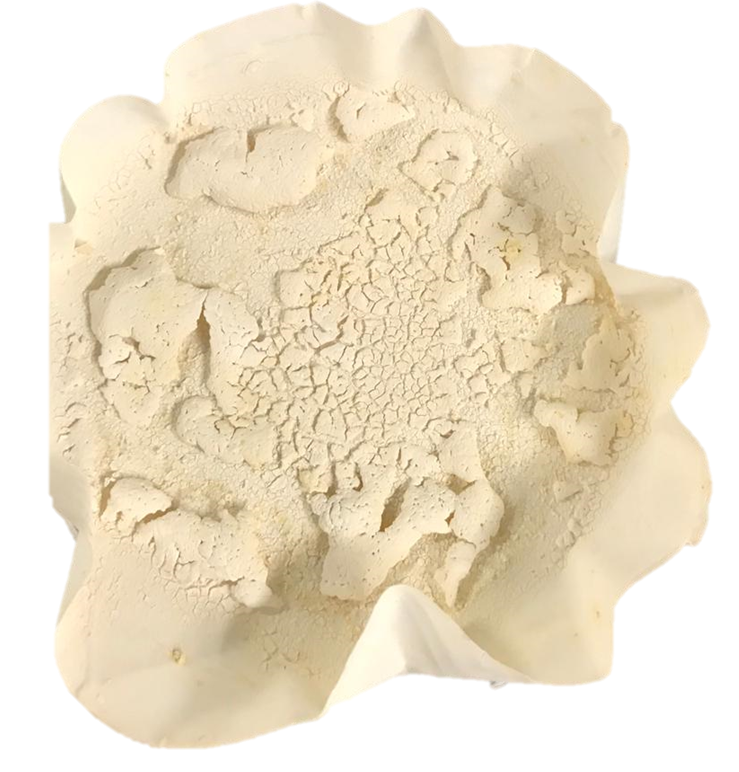
\includegraphics[width=0.3\linewidth]{Documento_Latex/Imagenes/capsulas.png}
    \caption{Silica microcapsules obtained by the methodology described in section \ref{sec:capusules}}
    \label{fig:capsules}
\end{figure}

\subsection{Film Elaboration} \label{sec:film_elaboration}
Once having 9g of nanocapsules, a masterbatch is prepared by mixing the nanocapsules load and polypropylene-maleic anhydride graft copolymer (PP-g-MAH) in a  20:80 mass proportion respectively. Before entering the sample into the internal mixer, this has to be preheated for 10 minutes so that it reaches a temperature of 190\degree C, after which the mix is poured and stays within 7 minutes at a speed of 60rpm. The material obtained must then be frozen to a temperature of -80\degree C for 3 hours. Afterward, it has to be taken into a blade mill for grinding for 2 minutes and in this way, the masterbatch is ready to be mixed with polypropylene homo-polymer (PP) to form the films. The quantity of masterbatch used is so that the nanocapsule load is 5\% of the total film weight. These two components go again through the same process of mixing as the masterbatch did. Finally, the process of compression molding is done by using a press. To do this, two aluminum foils and two Teflon foils are put over the two sides of the press, and in the inferior part of it, a quantity of 12g of the PP mixture is poured using a 19cm x 19cm x 3cm aluminum frame. The inferior and superior plates are both preheated to a temperature of 190\degree C and the press must be configured so that an initial pressure of 15 bar is applied during 1 minute and then a pressure of 110 bar must be applied during 1.5 minutes after which a 10 minutes cooling time is done. After this, the desired film of 19cm x 19cm with OS load is obtained (Figure \ref{fig:film}).

\begin{figure}[ht]
    \centering
    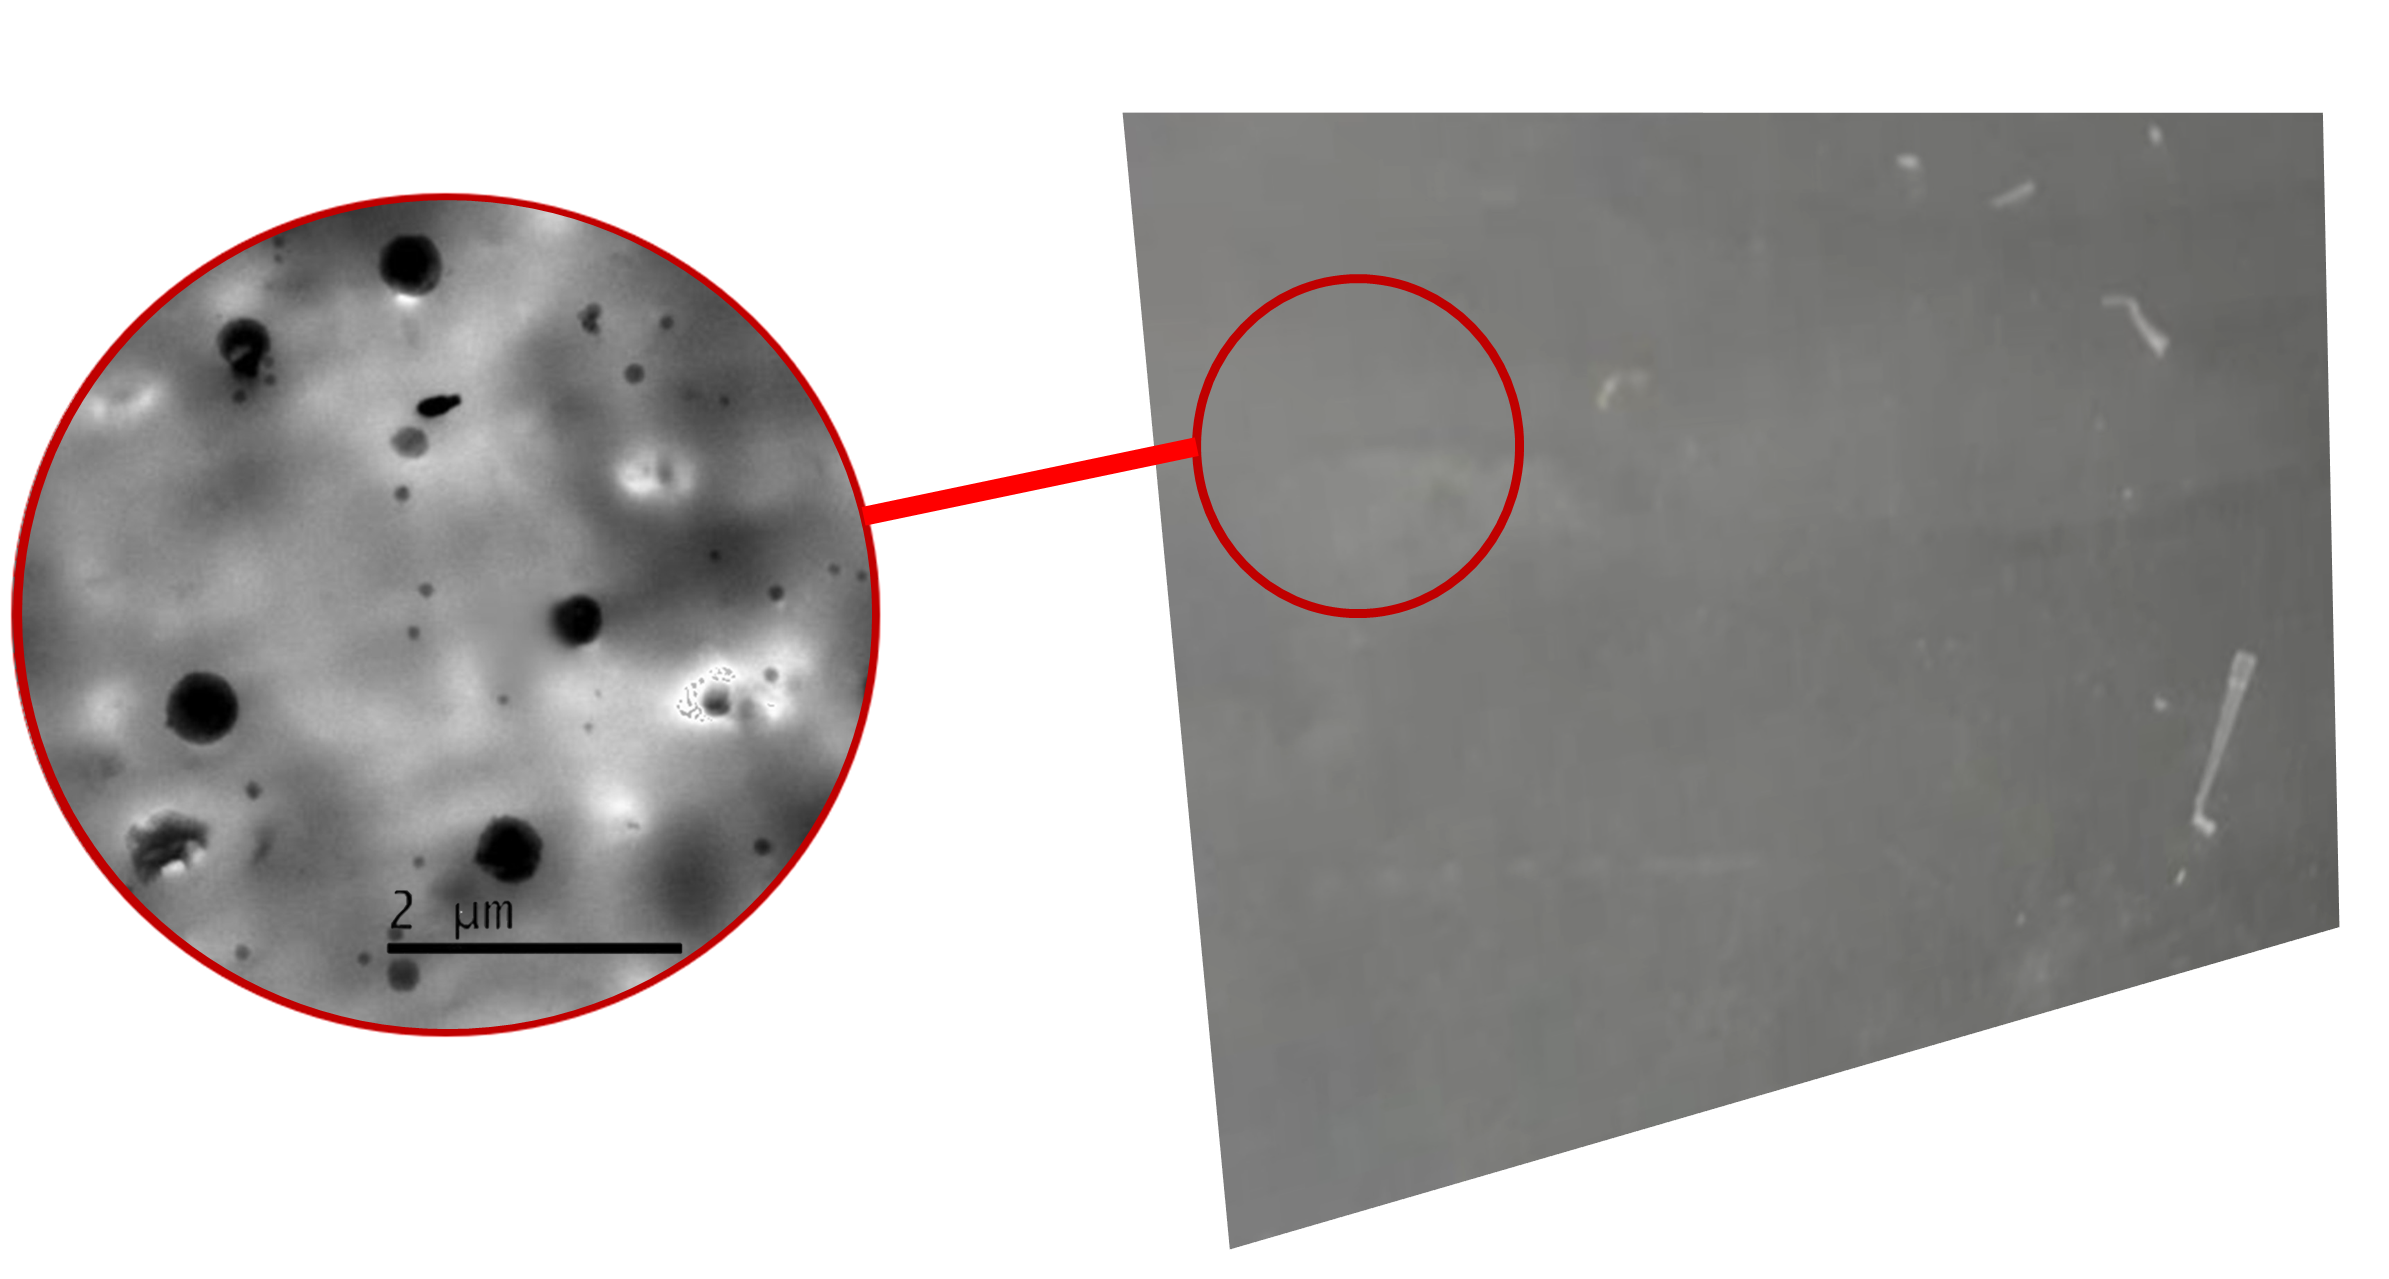
\includegraphics[width=0.6\linewidth]{Documento_Latex/Imagenes/pelicula.png}
    \caption{PP film containing silica microcapsules which were incorporated by the methodology described in section \ref{sec:film_elaboration} \cite{ArellanoAyala2019EfectosAntioxidantes}}
    \label{fig:film}
\end{figure}

\subsection{Headspace Oxygen Absorption Test}\label{subsec:headspace}
Head-space oxygen absorption is one of the two tests which enables to study the performance of the OS film, and its results together with the oxidative TGA are the ones that are used to verify the prediction capacity of the model proposed. To do this test, a Quantek 901 head-space oxygen analyzer was be used. First, a sample of the film made is placed within a 100mL glass bottle. This bottle is sealed by pressurizing its cap, after which it is ready to test. To perform the test, in the cap of the bottle, a plastic seal will be put and perforation with a needle will be made through it (See Figure \ref{fig:headspace}).

\begin{figure}[ht]
    \centering
    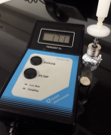
\includegraphics[width=0.25\textwidth]{Imagenes/headspace.png}
    \caption{Headspace oxygen absorption test}
    \label{fig:headspace}
\end{figure}

The gas extracted from the bottle goes by a syringe to a ''fuel cell" type oxygen sensor, which consists of a diffusion barrier, a sensing electrode made of platinum and a working electrode made of zinc, all submerged in a solution of potassium hydroxide which acts as an electrolyte \cite{Boissevain1996CorporateGuide}. The entering oxygen diffuses into the sensor a reduces to hydroxyl ions at the cathode.

 \reaction{O2 +2H2O +4e^- -> 4OH^-}
the hydroxyl ions formed are oxidized at the zinc anode.
 \reaction{2Pb + 4OH^- -> 2PbO +2H2O + 4e^-}
 which yields an overall cell reaction 
 \reaction{2Pb + O2 -> 2PbO}

 
 The current generated during this reaction is proportional to the concentration of oxygen present in the medium. With this in mind,  the sensor measures these currents and calculates the quantity of oxygen within the air \cite{GarciaMora2015KineticScavengers, Boissevain1996CorporateGuide}. This test was carried out every 12 hours until the oxygen concentration becomes constant in time, which indicates that the oxygen absorption on behalf of the film has stopped and so its useful life. It is essential to mention that for avoiding external air for entering the vial, each one of this was punctured once, and then it was discarded. Negative control was carried out for each head-space test done. For every puncture made, a  quantity of 4 ml of air is extracted from the bottle; this was calibrated, taking into account the advice from the manufacturer. The analyzer Quantek model 901 has a resolution of 0.1\% and an accuracy of $\pm$0.1\% in reading \cite{Instruments2019ModelAnalyzer}. 
 
\subsection{Oxidative TGA}
The second oxygen uptake performance test, which was made on OS films and linseed oil individually, is a thermogravimetric analysis (TGA). Given that in the autoxidation process described in Section \ref{subsec:PUFA_os}, there is an increase in the weight of oils due to the absorption of oxygen from the environment. Even though these changes in weight are minimal, they are big enough for being detected in the thermogravimetric analysis. So to determine the performance of the films and the oil, three TGA must be carried out. All tests were made using an SDT Q600 (TA instruments) with isothermal curves at 40\degree C, 60\degree C, 80\degree C, and 110\degree C and a heating rate of 20\degree C/min with a sample mas of 4 mg. The first TGA test carried out was under a nitrogen atmosphere. This is done to observe the sole effect of the flow of air around linseed oil and OS films. In this case, the volatile components within the sample are going to evaporate, generating a reduction in the measured mass. The second TGA test, which has to be carried is in a pure oxygen atmosphere. This is the case in which oxygen is in excess concerning the substrate, so the kinetics of oxidation can be simplified, as explained in section \ref{subsec:PUFA_os}. The results in the change of mass of the sample obtained are normalized for the mass reduction due to the evaporation obtained from the nitrogen atmosphere TGA. In this way, there is a guarantee that the changes observed in the mass on the oxygen TGA are exclusively due to the absorption of oxygen. The third and final TGA made was in air atmosphere, in which oxygen has a concentration of 21 vol\%. Contrary to the case of oxygen atmosphere TGA, in this case, it is not correct to assume that oxygen is in excess to the substrate in the oil, so the results obtained in this test must be compared to the complete autoxidation kinetics of the linseed oil.   

\section{Computational Methodology}\label{sec:computational methodology}
In this section of the document, an explanation of how the development of the computational tool was made is described. The first step taken towards fulfilling this objective was using conservation equations to establish a PDE which describes the dynamics of oxygen within linseed oil and OS polymeric films, this was developed both for monolayer films and for the multilayer films. Therefore, to evaluate the validity of the model developed, a new adjustment of the kinetic constant and initial concentrations was made over linseed oil kinetics. Once having determined the kinetic constants that describe the oxidation of linseed oil, a study of different numerical methods was made to find out which of these enabled a fast and accurate solution of the differential equations established from the mathematical models. Finally, once studied the method by which the model is solved, a graphic interface was developed so that an external user may study the effect of different parameters on the $O_2$ absorption. An explanation of how this interface was made is explained at the end of this section. 

\subsection{Model Description}\label{subsec:model_desc.}

\subsubsection{Mono Layer Film}
The main idea in developing a model that describes the oxygen uptake by an OS film is to replicate the results obtained experimentally by the Headspace oxygen test described in section \ref{subsec:headspace}. To establish this model, a film of Area $A$ and thickness $L$, which is inside a bottle volume $V$ and at constant temperature $T$ is considered. The gas in the bottle considered has an initial oxygen molar concentration $C_{ext_o}$. The situation described is shown in figure \ref{fig:model_diagram}. 

\begin{figure}[ht]
    \centering
    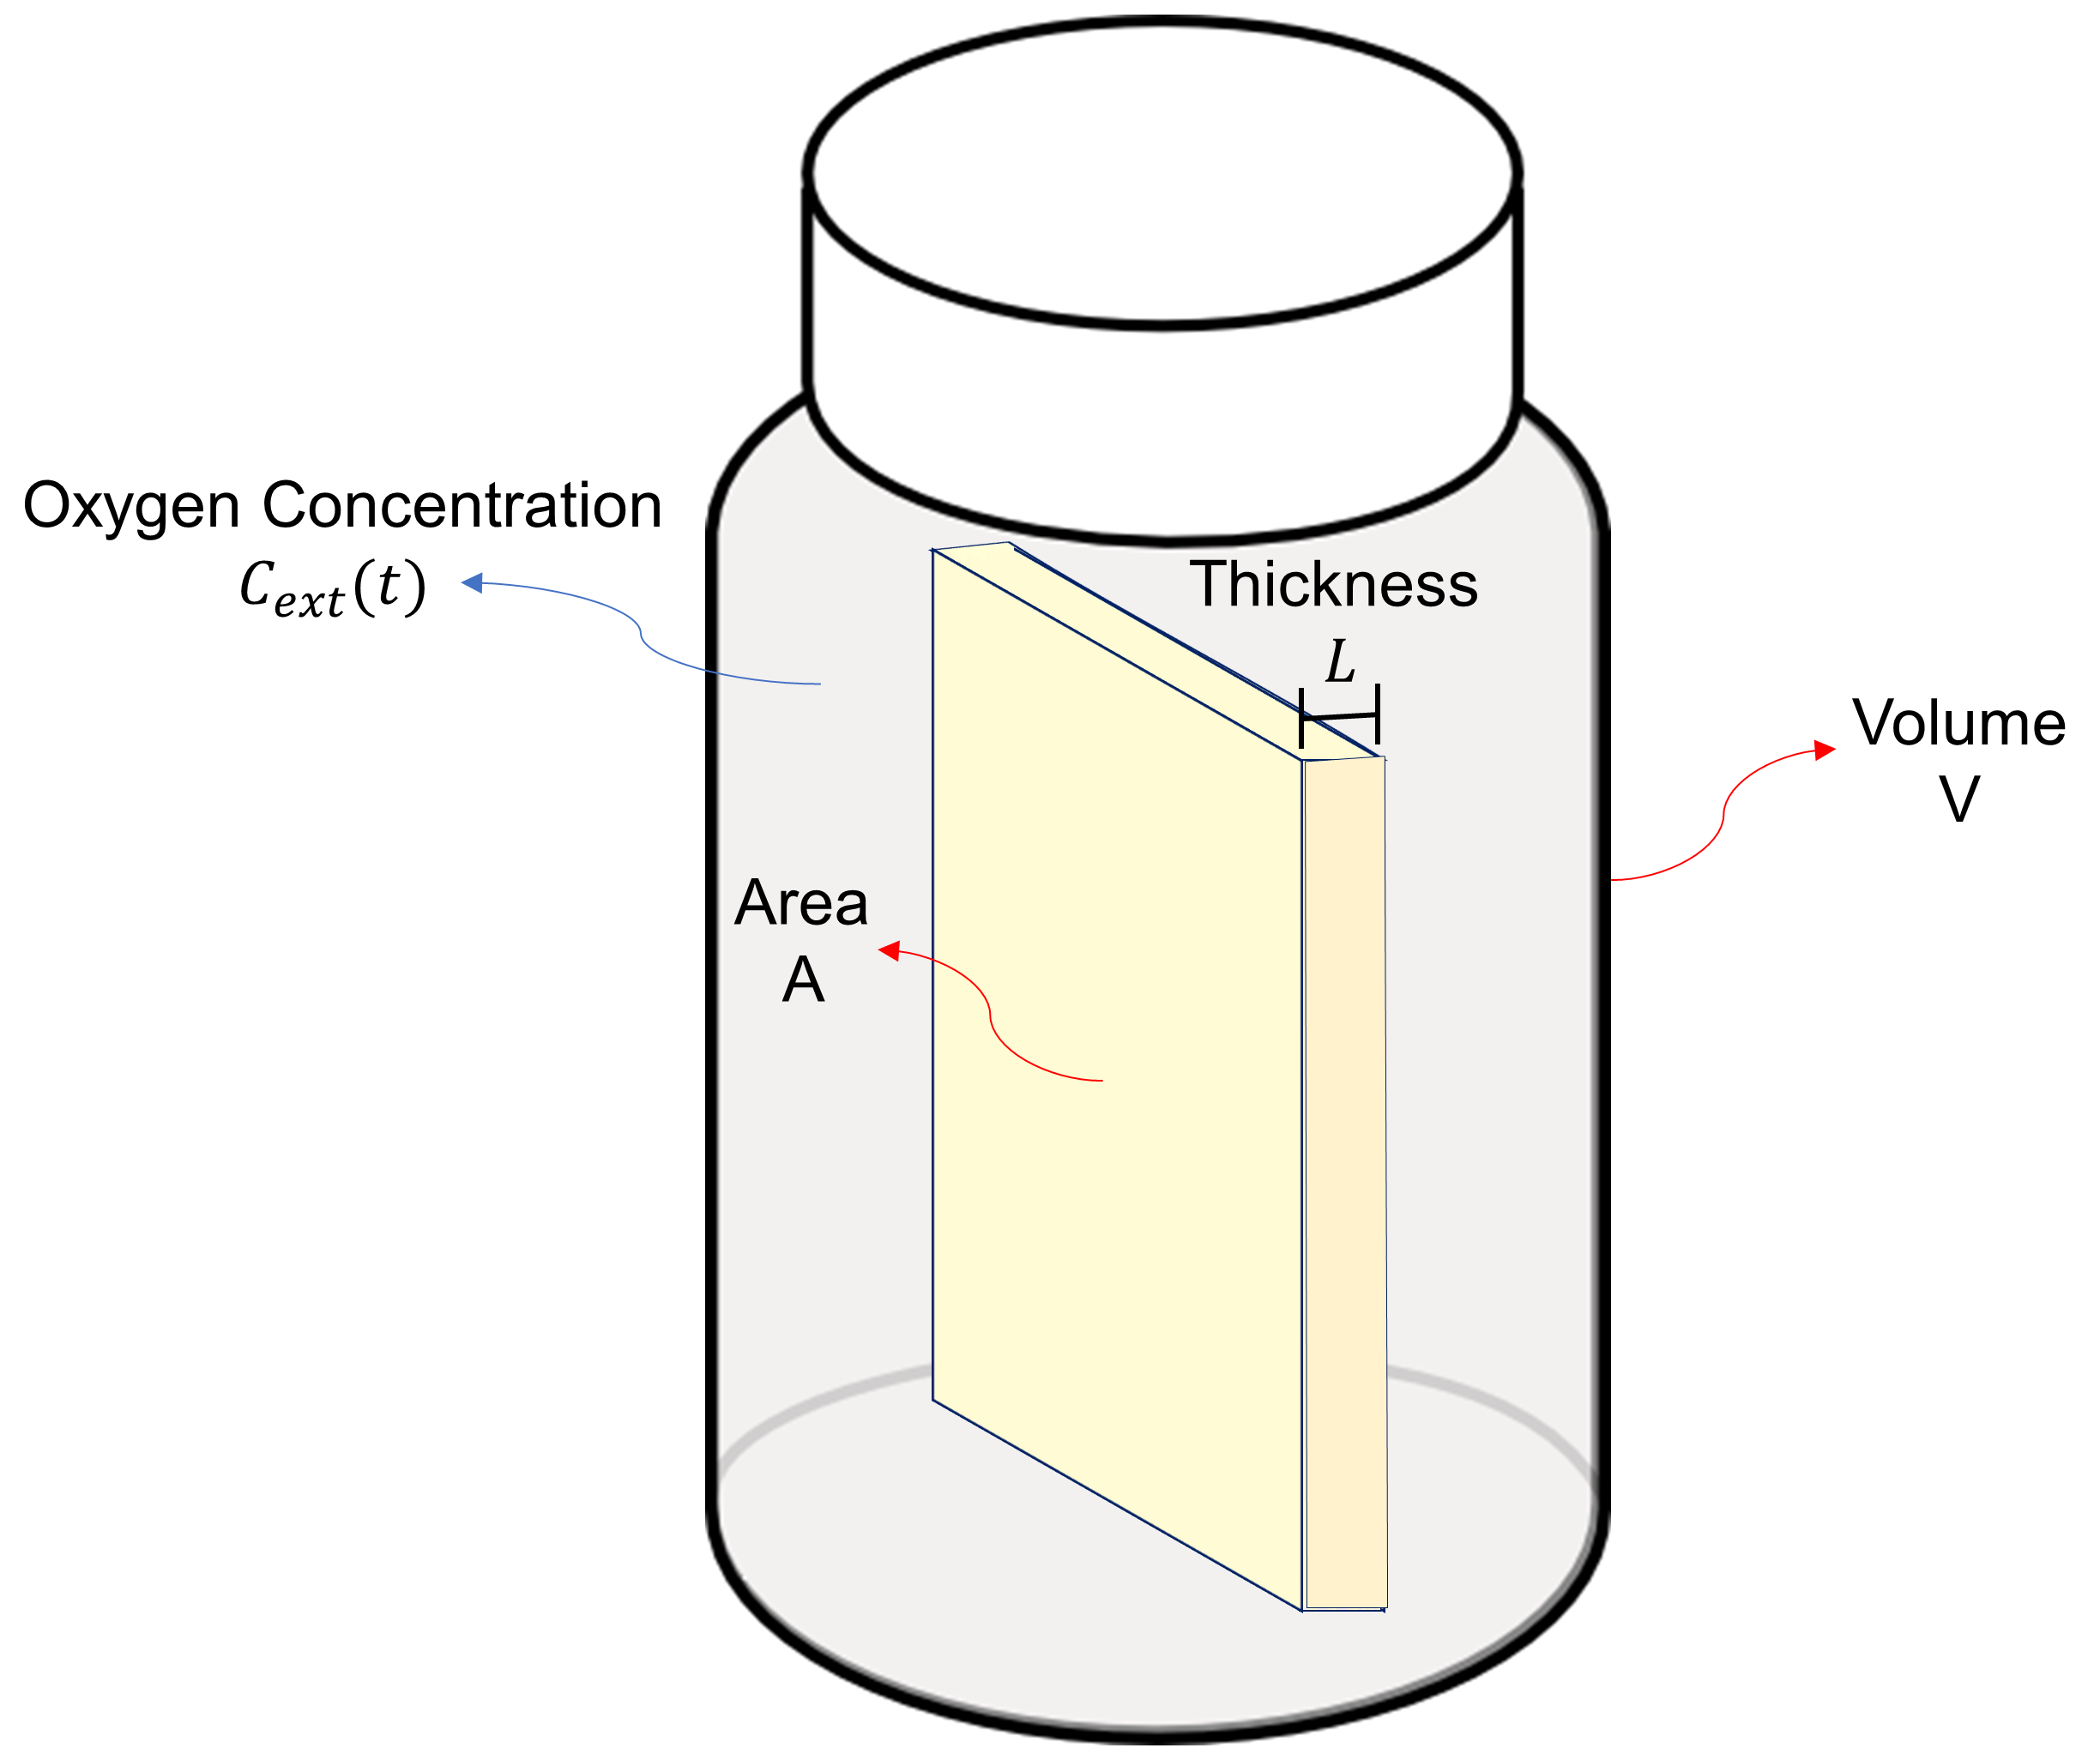
\includegraphics[width=0.5\linewidth]{Documento_Latex/Imagenes/modelo.png}
    \caption{Schematic diagram of the OS film in a vial with oxygen concentration $C_{ext}$}
    \label{fig:model_diagram}
\end{figure}

In this case, the homogeneous film approach is going to be used. This considers the whole film as reactive with an initial OS volumetric concentration $C_{OS_0}$. For the initial conditions of the model, it was assumed that there is no oxygen consumption or diffusion in the process of compression molding, which is why the initial molar concentration of oxygen in the film is $[O_2]=0 \hspace{5pt} mol/cm^3$.  It is essential to state that in this model, oxygen will be assumed to enter by both faces of Area $A$ and given that this area is much bigger than the thickness $L$ of the film, then the propagation of oxygen into the foil can be assumed to be one dimensional in the direction normal to its faces (Figure \ref{fig:model_diagram}).

Now assuming that the film is isotropic, the diffusion of oxygen through it is going to be given by Fick's first law, which allows calculating the molar diffusive flux as the product of the diffusivity of oxygen in the polymer and the gradient of the $O_2$ concentration within the film (Equation \ref{eq:flux}).

\begin{equation}
    J=-D_{O_2}\nabla [O_2] \xrightarrow{1D}J_x=-D_{O_2}\frac{\partial [O_2]}{\partial x}
    \label{eq:flux}
\end{equation}

In the previous equation, $J$ represents the molar flux of oxygen and $D$ is the diffusivity of oxygen in the polymer material which the film is made of. The equation stated before indicates that the flux will go in the direction in which the concentration of $O_2$ decreases; this suggests that the mass will move towards reducing the concentration gradient in the system. Now, applying this to the oxygen molar balance, the equation \ref{eq:mass_bal_dif} is obtained. 

\begin{equation}
    \frac{\partial [O_2]}{\partial t}= -\nabla \cdot J= \frac{\partial}{\partial x} \left(D_{O_2}\frac{\partial [O_2] }{\partial x}\right)
    \label{eq:mass_bal_dif}
\end{equation}

This last equation is the transient diffusion equation and describes how any species propagates in a medium given a gradient in its concentration. In this case, given that the film is assumed to be reactive, a source/sink term must be taken into account in the prior equation due to the consumption of oxygen by the OS.

\begin{equation}
    \frac{\partial [O_2]}{\partial t}= \frac{\partial}{\partial x} \left(D_{O_2}\frac{\partial [O_2] }{\partial x}\right)+ R
    \label{eq:mass_bal_dif_reacc}
\end{equation}

The equation \ref{eq:mass_bal_dif_reacc}, corresponds to the one dimensional transient diffusion-reaction equation, in which $R$ represents the reactive term. By describing mass conservation in the system with equation \ref{eq:mass_bal_dif_reacc}, there is an assumption that no convection occurs within the vial so there is no net flow of the oxygen in the polymeric film and the only movement of this specie is given by concentration gradients. Now to describe the reactive term shown in the last equation, the kinetic model presented by Garcia \cite{GarciaMora2015KineticScavengers} for describing linseed oil autoxidation is going to be used with a modification on the termination equation of peroxyl radicals (this modification is explained in section). This model assumes that the reactions which occurs during oxidation are:

\reaction[reacc:initiation]{2ROOH ->[k_1] ROO^. +R^. + carbonyl + Scission}
\reaction[reacc:O_2 consumption]{R^. + O2 ->[k_2] ROO^.}
\reaction[reacc: propagation]{ROO^. + RH ->[k_3] ROOH + R^.}
\reaction[reacc:termination_2alkyrad]{R^. +R^. ->[k_4] $\text{Inactive Products}$}
\reaction[reacc:termination_alky_peroxide_rad]{R^. +ROO^. ->[k_5] $\text{Inactive Products}$}
\reaction[reacc:termination_2peroxide_rad]{ROO^. +ROO^. ->[k_6] $\text{Inactive Products}$}

Where $ROOH$ is hydroperoxide, $RH$ is the substrate and \ce{R^.}, \ce{ROO^.} are the alkyl and peroxyl radicals respectively. By assigning a simple kinetics using the rate law expression the following system of ordinary differential equations (ODE) is obtained:

\begin{gather}
    \frac{d[\ce{R^.}]}{dt}= k_1[ROOH]^2 - k_2 [\ce{R^.}][O_2]+ k_3[\ce{ROO^.}][RH]-2k_4[\ce{R^.}]^2 -k_5[\ce{R^.}][\ce{ROO^.}]\label{eq:consum_R.}\\
    \frac{d[\ce{ROO^.}]}{dt}= k_1[ROOH]^2 + k_2 [\ce{R^.}][O_2]- k_3[\ce{ROO^.}][RH]-k_5[\ce{R^.}][\ce{ROO^.}]-2k_6 [ROO^.]^2\\
   \frac{d[ROOH]}{dt}= -2k_1[ROOH]^2 + k_3[\ce{ROO^.}][RH]\\
   \frac{d[RH]}{dt}=-k_3[\ce{ROO^.}][RH]\label{eq:consum_RH}\\
   \frac{d[O_2]}{dt}= -k_2[\ce{R^.}][O_2]\label{eq:consum_O2}
\end{gather}

Combining the equations \ref{eq:mass_bal_dif_reacc} and \ref{eq:consum_O2}, the oxygen mass balance can be expressed as:

\begin{equation}
     \frac{\partial [O_2]}{\partial t}= \frac{\partial}{\partial x} \left(D_{O_2}\frac{\partial [O_2] }{\partial x}\right) -k_2[\ce{R^.}][O_2].
    \label{eq:mass_bal_def}
\end{equation}

This last equation together with equations \ref{eq:consum_R.} to \ref{eq:consum_RH} are going to describe the dynamics of oxygen concentration within the film. Also, this are the ones that are going to be numerically solved (this is going to be explained in section \ref{subsec:numerical_methodology.}). On the other hand, the total quantity of oxygen absorbed by the film is calculated by integrating the mass flow of oxygen into it. 

\begin{equation}
    m_{O_2}(t)= \int_0^t \dot{m}dt =M_{O_2}A\int_0^t Jdt 
\end{equation}

To arrive at the right-hand side of the equation, mass flux was calculated by multiplying the molar flux $J$ by the molecular weight of oxygen $M_{O_2}$, while the mass flow was calculated by multiplying the mass flux by the film area $A$. It is essential to state that the flux $J$ used to calculate the total mass of oxygen in the film is the sum of the flux at both faces of the film, $J= J_x\rvert_{x = 0} - J_x\rvert_{x = L}$. But given that the concentration $[O_2]$ is symmetrical concerning the film, the flux at both faces will be equal in magnitude, so $J=2J_x\rvert_{x = 0}$.  Now replacing the definition of molar flux (Equation \ref{eq:flux}) into the previous expression

\begin{equation}
    m_{O_2}(t) =-2D_{O_2}AM_{O_2}\int_0^t \frac{\partial [O_2]}{\partial x}\biggr\rvert_{x = 0}dt
    \label{eq:total_mass_O2}
\end{equation}

This last expression will enable to calculate the oxygen uptake profile through time as well as the head space oxygen concentration profile (Equation \ref{eq:headspace}). 

\begin{equation}
    C_{ext}(t)= C_{ext_o} - \frac{1}{M_{O_2}V} m_{O_2}(t)= C_{ext_o} + \frac{2AD_{O_2}}{V} \int_0^t \frac{\partial [O_2]}{\partial x}\biggr\rvert_{x = 0}dt
    \label{eq:headspace}
\end{equation}

This last quantity, $C_{ext}(t)$, is of great interest,
because it is the one that the headspace test
allows to obtain experimentally, so the model
will seek to predict the behavior of this quantity
overtime. Concerning the initial and boundary conditions in this problem, as stated at the beginning of this section the film is going to be considered to be devoid of $O_2$ and the external headspace oxygen concentration is going to be $C_{ext_o}$. Also concerning the initial concentration of the reacting species in the linseed oil (i.e. hydroperoxide,substrate, alkyl, and hydroxyl radicals) is it assumed that they are going to be uniform through the whole film (Equation \ref{eq:ic_mono_film}). 

\begin{align}
    &\text{IC: } & &[O_2](x,t=0)=0, & &C_{ext}(t=0)= C_{ext_o},\nonumber\\
    && &[\ce{RH}](x,t=0)=C_{OS}[\ce{RH}]_o,   & &[\ce{ROOH}](x,t=0)=C_{OS}[\ce{ROOH}]_o, \nonumber\\
    && &[\ce{R^.}](x,t=0)=C_{OS}[\ce{R^.}]_o,   & &[\ce{ROO^.}](x,t=0)=C_{OS}[\ce{ROO^.}]_o. 
    \label{eq:ic_mono_film}
\end{align}
    
The quantities $[\ce{RH}]_o$, $[\ce{ROOH}]_o$,  $[\ce{R^.}]_o$, and $[\ce{ROO^.}]_o$ are the respective molar concentrations of chemical species in Linseed oil and $C_{os}$ is the charge of OS scavenger in the film. This latter quantity is calculated by multiplying the mass charge of OS in the film (wt\%) by the reason between the oil and the film density (Equation \ref{eq:load_concentration}).

\begin{equation}
    C_{OS}= \text{Oil wt}\% \frac{\rho_{polymer}}{\rho_{oil}}
    \label{eq:load_concentration}
\end{equation}

On the other hand, given that the molar balance of oxygen in the film has second-order derivative respect to the spatial component, it is necessary to establish two boundary conditions over the film so that the problem stated has a solution. These conditions are given in the outer face of the film, which is in contact with the head-space gas. In this case, oxygen dissolved in the boundary face of the film must be in equilibrium with the external oxygen. This equilibrium is described by Henry's law which states that the partial concentration of the oxygen dissolved in the polymer is proportional to the partial pressure of oxygen in the head-space gas (i.e. $[O_2](x=0, L)=s\hspace{2pt}p_{O_2}$ ). The relation between the partial pressure of oxygen and its'external concentration is obtained assuming that the gas in the vial behaves as an ideal gas.  In that case $p_{O_2}=RTC_{ext}(t)$, and so the boundary conditions for oxygen concentration in the film are:

\begin{align}
    &\text{BC:} & &[O_2](x=0, t)= \left(sRT\right) C_{ext}(t) & & [O_2](x=L, t)= \left(sRT\right) C_{ext}(t)
    \label{eq:bc_mono_film}
\end{align}

With these set of initial and boundary conditions, the complete set of conditions necessary to solve the problem is established.

\subsubsection{Multi-layer Film}
Continuing with the presentation of the mathematical models developed for the creation of an OS film modeling tool, the case of a multilayer system was considered. The situation studied was a multilayer OS film with total thickness $L$,  composed of  $n$ layers, each one of thickness $L_i, 0<i<n$ where  $L_i\neq L_j, \forall  i\neq j$ and made of a different material. The film has a face of area $A$ and is inside a vial of volume $V$ with an initial headspace oxygen concentration $C_{ext_o}$. The situation described is shown in figure \ref{fig:model_multilayer_diagram}.

\begin{figure}[ht]
    \centering
    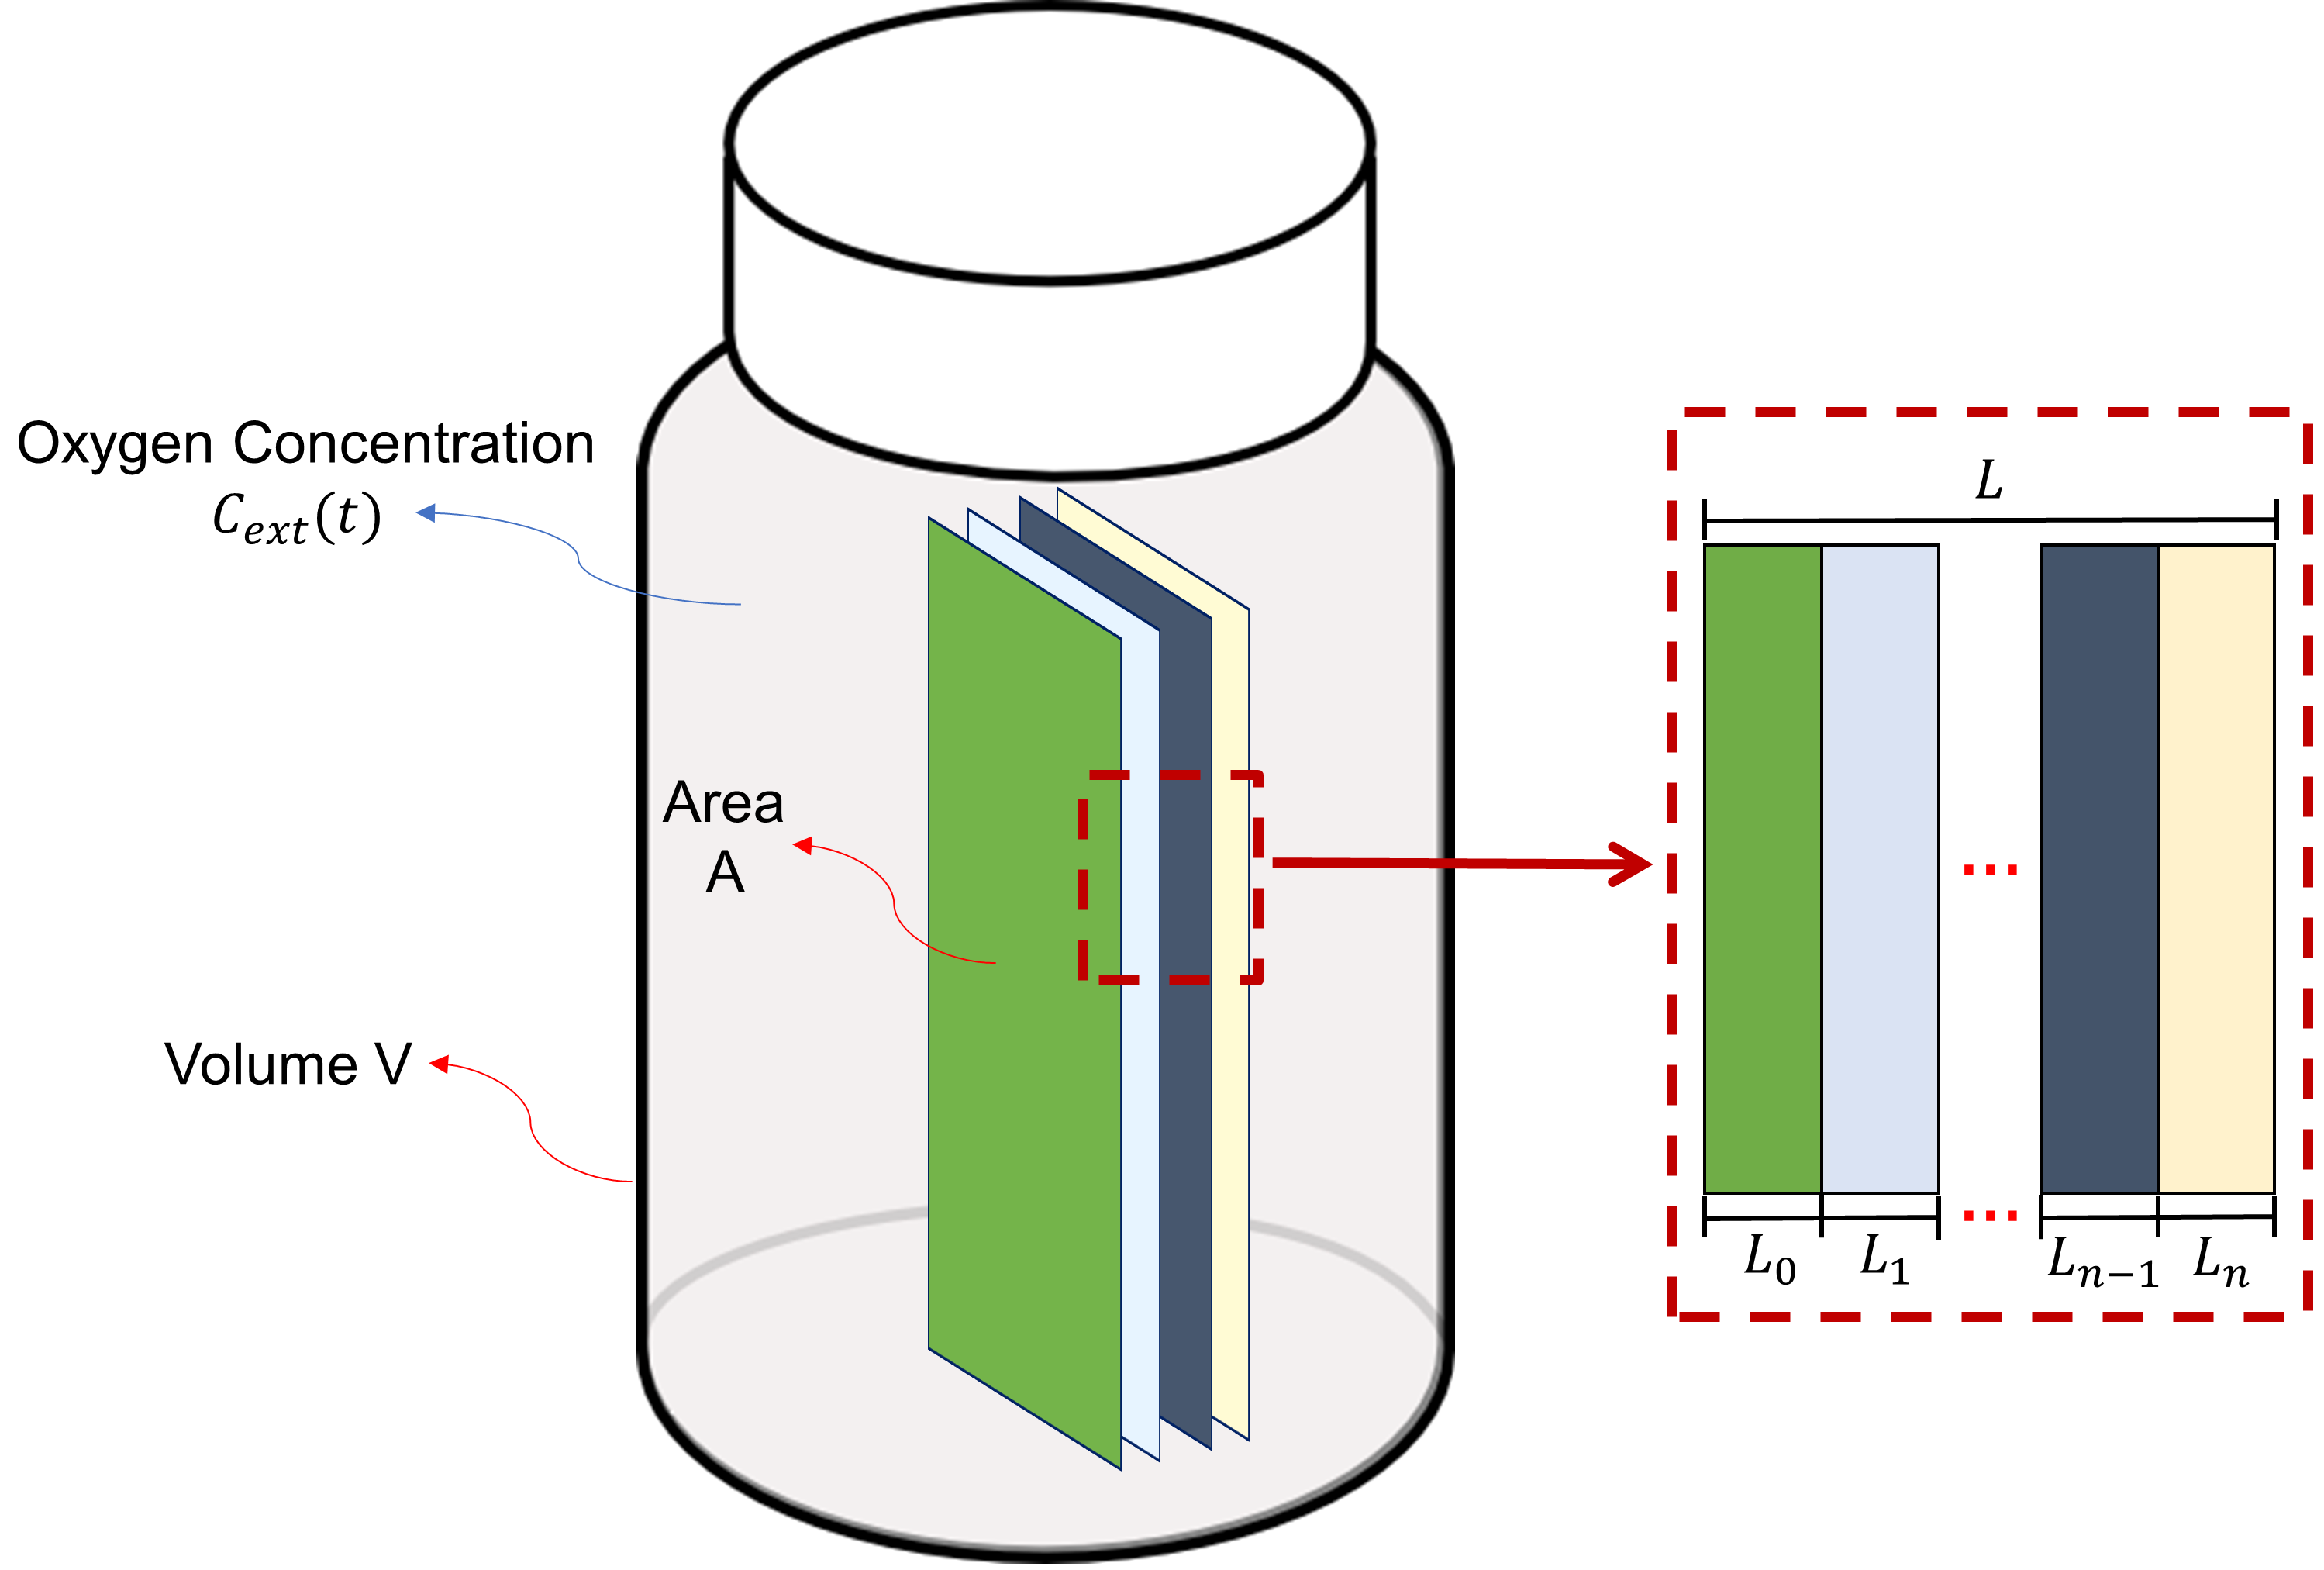
\includegraphics[width=0.62\linewidth]{Documento_Latex/Imagenes/modelo_multicapa.png}
    \caption{Schematic diagram of a OS film composed of $n$ different layers in a vial with oxygen concentration $C_{ext}$}
    \label{fig:model_multilayer_diagram}
\end{figure}

The equation describing the dynamics of the reaction in the film are the same as equations \ref{eq:consum_R.} to \ref{eq:consum_RH}, while the expression regarding oxygen concentration dynamics in the film is going to be

\begin{equation}
    \frac{\partial [O_2]}{\partial t}= \frac{\partial}{\partial x} \left(D_{O_2}(x) \frac{\partial [O_2] }{\partial x}\right) -k_2[\ce{R^.}][O_2]
    \label{eq:mass_bal_def_multi}
\end{equation}

The main difference between the last equation and equation \ref{eq:mass_bal_def} is that the diffusivity of oxygen depends on the position $x$ in the film. The function that describes this dependence is :

\begin{align}
    D_{O_2}&=  D_i,  & L_{i-1}&< x< L_i,
\end{align}

where $D_i$ is the diffusivity of oxygen in the material of the $i$th-layer of the film. Now, given that the model assumes that all layers are of  different materials, then the flux of oxygen in both faces of the film is not going to be equal, i.e. $J_x\rvert_{x = 0}\neq-J_x\rvert_{x = L} $. This is why in this case the total oxygen mass absorbed by the film has to be calculated as:
\begin{equation}
    m_{O_2}(t) =-AM_{O_2}\int_0^t \left(D_{O_2}(x)\frac{\partial [O_2]}{\partial x}\biggr\rvert_{x = 0} -D_{O_2}(x)\frac{\partial [O_2]}{\partial x}\biggr\rvert_{x = L}\right )dt.
    \label{eq:total_mass_O2_multi}
\end{equation}

And so the headspace oxygen concentration profile is going to be given by:
\begin{equation}
    C_{ext}(t)=C_{ext_o} + \frac{A}{V} \int_0^t \left(D_{O_2}(x)\frac{\partial [O_2]}{\partial x}\biggr\rvert_{x = 0} -D_{O_2}(x)\frac{\partial [O_2]}{\partial x}\biggr\rvert_{x = L}\right) dt.
    \label{eq:headspace_multi}
\end{equation}

Besides the previous equations, there exists an internal boundary condition at the interface between any two collateral layers. This states that the flux of oxygen as well as it's partial pressure are continuous due to mass conservation. The partial pressure of a gas dissolved in a certain media is given by Henry's law, $p=sC$, where $s$ is the solubility of the gas in the media. Given that at the interface of the layer the partial pressure must be continuous:
 \begin{equation}
   p_{i}(x=L_i) =p_{i+1}(x=L_i)  \xrightarrow{}\frac{[O_2]_{i}(x=L_i)}{S_{i}} =\frac{[O_2]_{i+1}(x=L_i)}{S_{i+1}},
 \end{equation} where $p_{i}(x=L_i)$, $[O_2]_{i}(x=L_i)$ and $S_{i}$ is the partial pressure, concentration and solubility of oxygen in $ith$ layer of the film at position $x=L_i$ (which is the interface) and  $p_{i+1}(x=L_i)$, $[O_2]_{i+1}(x=L_i)$ and $S_{i+1}$ are the partial pressure, concentration and solubility of oxygen in the $i+1th$ film of the layer at the interface $x=L_i$. 

Lastly, to establish this model, boundary and initial conditions are necessary. For the latter conditions, this are the same ones established for the monolayer film (Equation  \ref{eq:ic_mono_film}) with the difference that $C_{OS}=f(x)$ (see equation \ref{eq:ic_multi_film}).

\begin{align}
    &\text{IC: } & &[O_2](x,t=0)=0, & &C_{ext}(t=0)= C_{ext_o},\nonumber\\
    && &[\ce{RH}](x,t=0)=C_{OS}(x)[\ce{RH}]_o,   & &[\ce{ROOH}](x,t=0)=C_{OS}(x)[\ce{ROOH}]_o, \nonumber\\
    && &[\ce{R^.}](x,t=0)=C_{OS}(x)[\ce{R^.}]_o,   & &[\ce{ROO^.}](x,t=0)=C_{OS}(x)[\ce{ROO^.}]_o. 
    \label{eq:ic_multi_film}
\end{align}

The reason why in this case $C_{OS}$ depends on the position of film is that not all the layers of the film are reactive. The layers which are inert, have no load of Linseed oil, while reactive layers are. This do not necessarily mean that  all have the same load of Linseed oil (i.e. $C_{OS_i}\neq C_{OS_{j}}, \forall i\neq j$). With this in mind, $C_{OS}(x)$  is given by the following expression:
\begin{equation}
    C_{OS}(x)= 
    \begin{cases}
    0  &\quad\text{if film }i \text{ is inert and } L_{i-1} \le x \ge L_i\\
    C_{OS_i}  &\quad\text{if film }i \text{ is reactive and }  L_{i-1} \le x \ge L_i,\\
    \end{cases}
\end{equation}
where $C_{OS_i}$ (the load of OS per layer) is calculated as:
\begin{equation}
    C_{OS_i}= \text{Oil wt}\%_i \left( \frac{\rho_{polymer_i}}{\rho_{oil}}\right).
    \label{eq:load_multi_concentration}
\end{equation}

On the other hand, the boundary conditions established for the monolayer film (Equation \ref{eq:bc_mono_film}) are valid for the multilayer case, with the difference that the solubility term on each boundary depends on the material of the exterior faces. Having said this, the boundary condition are going to be:
\begin{align}
    &\text{BC:} & &[O_2](x=0, t)= \left(s_0RT\right) C_{ext}(t) & & [O_2](x=L, t)= \left(s_nRT\right) C_{ext}(t),
    \label{eq:bc_multi_film}
\end{align}
where $s_o$ and $s_n$ are the oxygen solubility in the material of the first and last layer of the film. With the boundary and initial conditions established, the model for the multilayer film case is finished. 

\subsection{Numerical Resolution Methodology}\label{subsec:numerical_methodology.}
To obtain a solution to the models presented in section \ref{sec:modeling}, given the complexity of the system of differential equations to be solved, there exists the necessity of using numerical methods. Even though these methods do not enable us to find the exact solution of the problem, it does enables us to obtain an approximation of the analytical solution within an error interval, which depends on the implementation of the solution algorithm. In this case, given that the system of partial differential equations (PDE) which is needed to be solved is one dimensional, this system is going to be solved using finite differences techniques. These methods are based on the approximation of the definition of derivative to a finite difference, which can be solved algebraically (Equation \ref{eq:fin_dif}).

\begin{equation}
    \frac{df}{dx}\approx \frac{f(x_{i+1})-f(x_{i}) }{\Delta x}
    \label{eq:fin_dif}
\end{equation}

To use this technique, the domains in which the equations are going to be solved must be discretized. With this in mind, the spacial domain $x$ in which the diffusion and reaction of oxygen take place becomes $x_i$, which are $n$ discrete points that represent the whole domain. In the same way, time $t$ becomes $t_j$ where $0<j<m$, being $m$ the total number of steps taken in the time interval which is going to be solved. For solving the  system of equations \ref{eq:consum_RH} to  \ref{eq:mass_bal_def}
different finite-difference algorithms were evaluated to find which of these methods was able to solve the diffusion-reaction equation in a fast and stable way. In the next subsections, the methods which were taken into account for this are going to be described, as well as how these were applied to the PDE system of the OS film. 

\subsubsection{Methods of lines}
One of the most straightforward techniques used for numerically solving PDEs is the method of lines (MOL). This method enables to transform a system of PDEs to a system of ODEs, which in turn can be solved using ODE methods such as Runge-Kutta or backward difference formula (BDF), among others. To do this all the dimensions within the PDE equation must be discretized except one. In this case, the equation which is going to be solved is

\begin{equation*}
     \frac{\partial [O_2]}{\partial t}= \frac{\partial}{\partial x} \left(D_{O_2}\frac{\partial [O_2] }{\partial x}\right) -k_2[\ce{R^.}][O_2]
\end{equation*}

The variable which is going to be discretized is $x$ or the spacial dimension. This was chosen given that the only specie which has a spacial component in its mass balance is oxygen, the rest only varies along time. This implies that the reactive sites are fixed within the film. The discretization scheme chosen for the second derivative is a second-order central difference  (Equation \ref{eq:disc_diff}). 

\begin{equation}
    D_{O_2}\frac{\partial^2 [O_2]}{\partial x^2}= D_{O_2} \frac{[O_2]_{i-1}-2[O_2]_{i}+[O_2]_{i+1}}{(\Delta x)^2}
    \label{eq:disc_diff}
\end{equation}

Applying the previous equation into molar balance equation of oxygen the next expression is obtained:
\begin{equation}
     \frac{\partial [O_2]_i}{\partial t}=  D_{O_2} \frac{[O_2]_{i-1}-2[O_2]_{i}+[O_2]_{i+1}}{(\Delta x)^2} -k_2[\ce{R^.}]_i[O_2]_i.
     \label{eq:LOD_oxygen}
\end{equation}
This equation now represents an ordinary differential equation for $[O_2]_i$, which is a vector of variables of concentration of oxygen through the spacial domain which only depends on time (see Figure \ref{fig:LOD_diagram}).

\begin{figure}[ht]
    \centering
    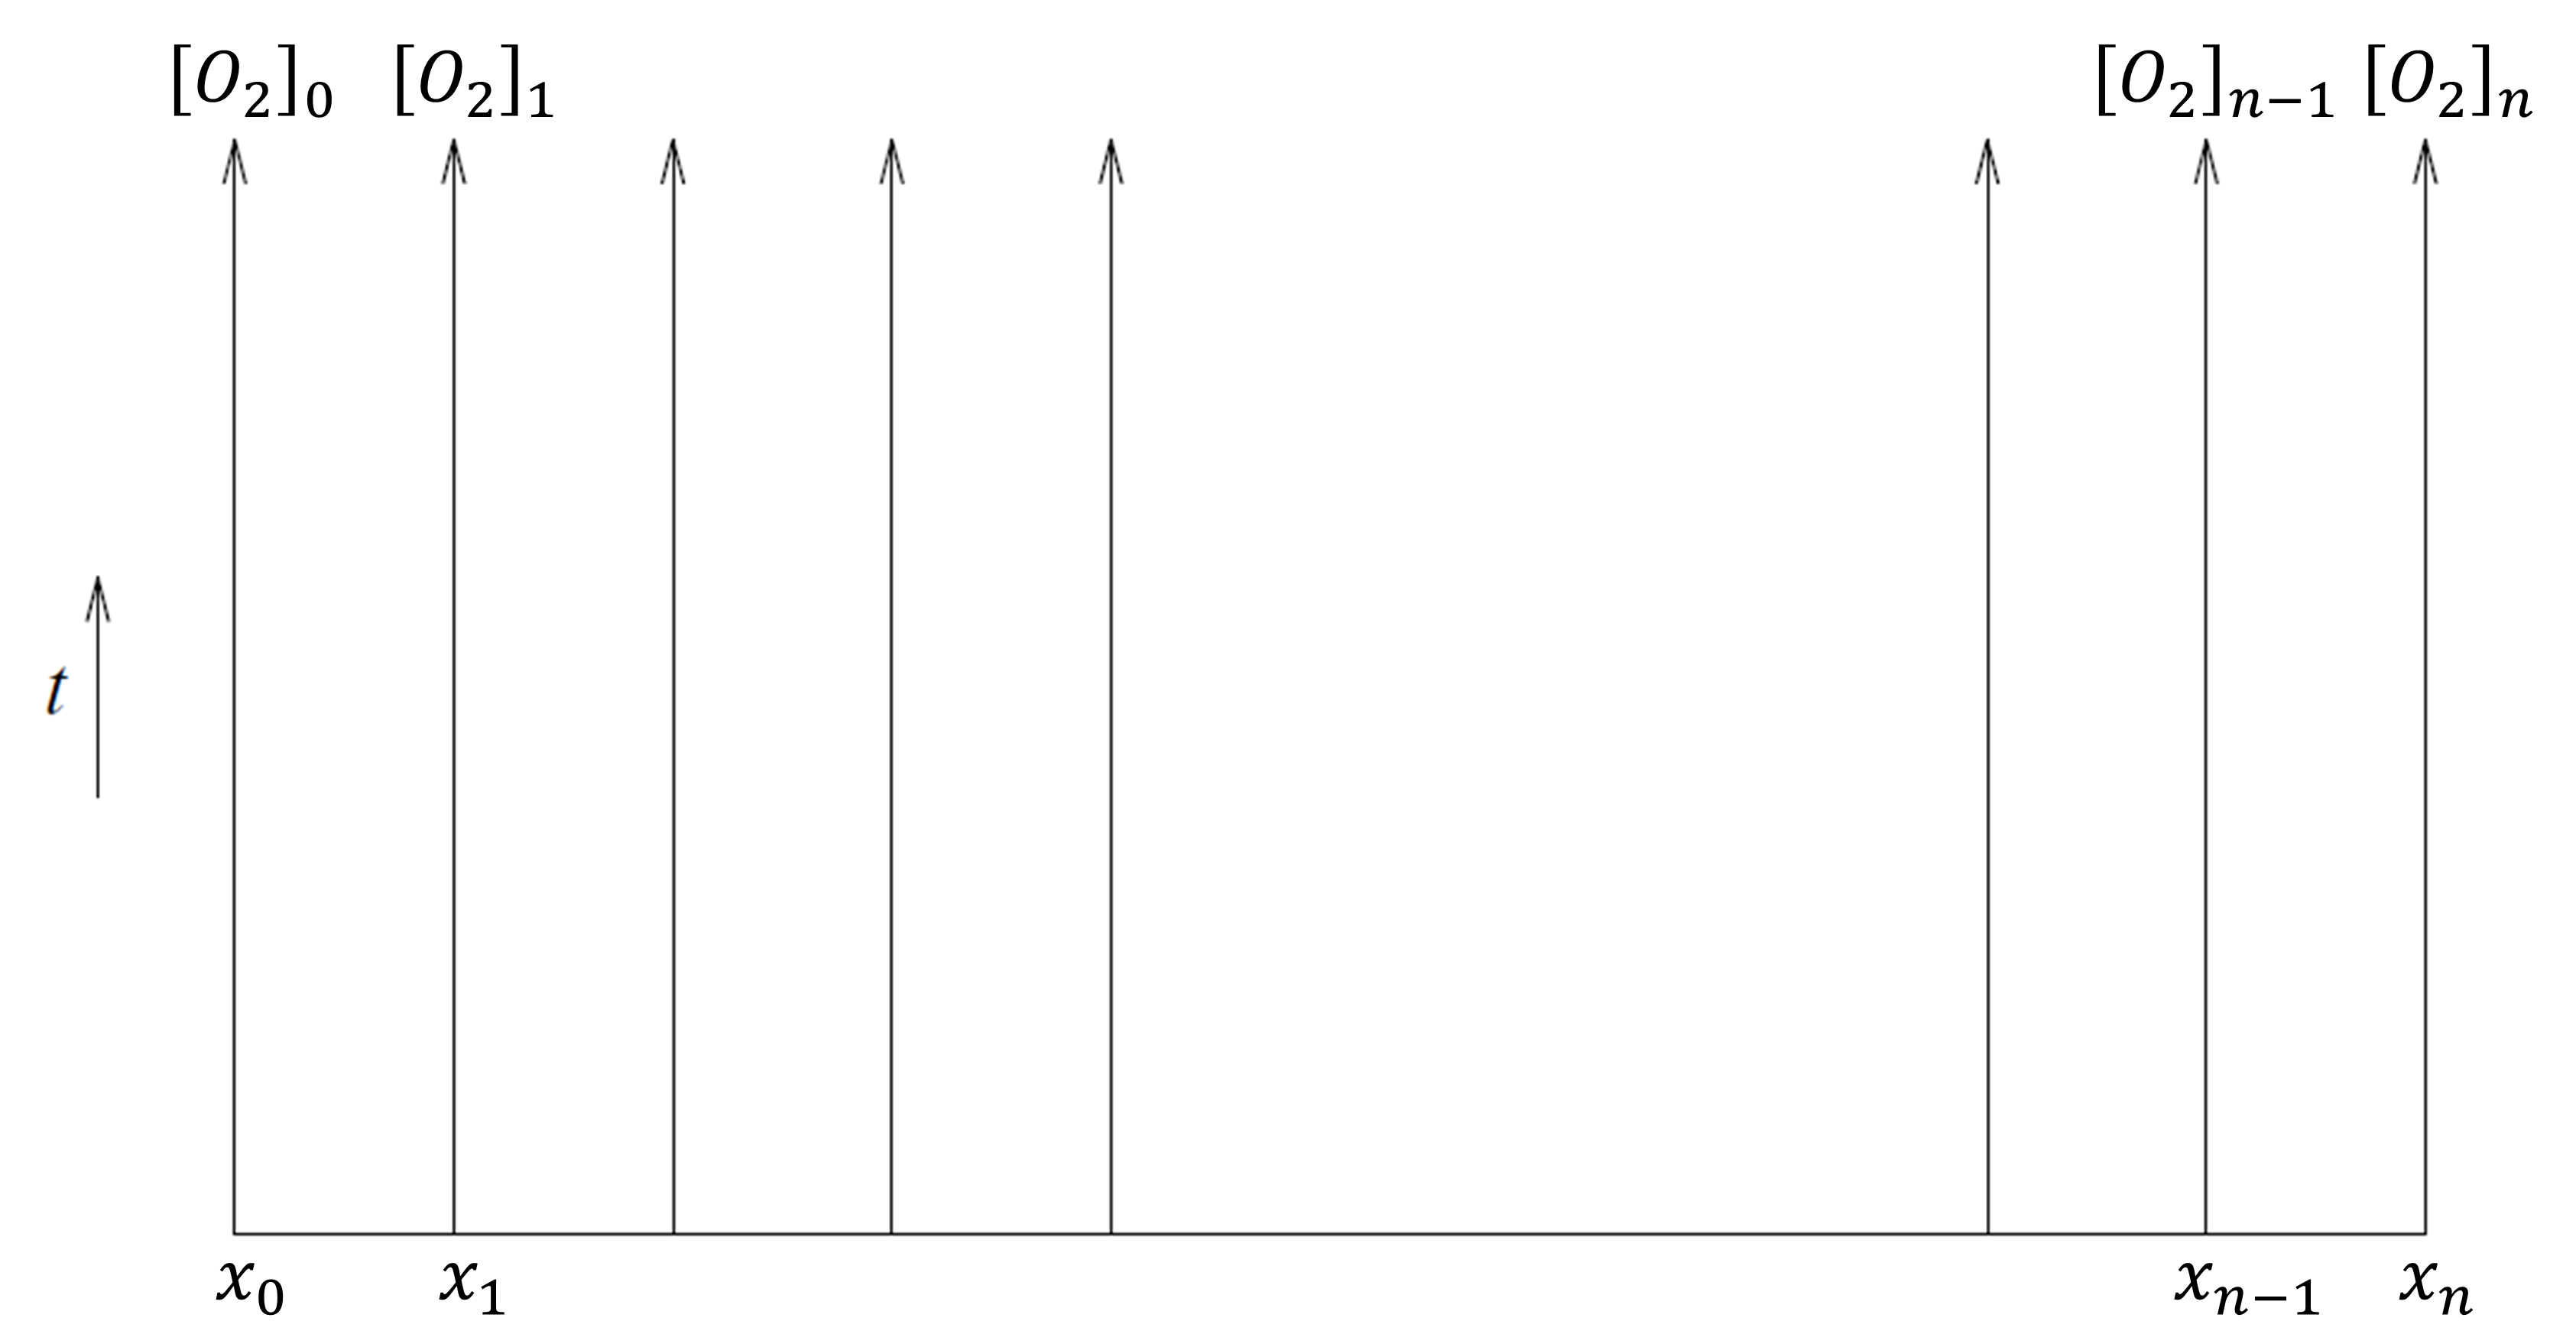
\includegraphics[width=0.7 \linewidth]{Documento_Latex/Imagenes/LOD.png}
    \caption{Method of lines interpretation. $[O_2]_i$ is the solution along the line forward in time at the grid point $x_i$. Adapted from \cite{LeVeque2007FiniteProblems}.}
    \label{fig:LOD_diagram}
\end{figure}

To solve the system of ODEs, a trapezoidal method will be used. These methods consist of calculating the time derivative at a point $t_i$ as the average of the derivative in that time step and the derivative in the next time step $t_{i+1}$. With this in mind, if the derivative of the oxygen concentration in the film with respect to time is given by equation \ref{eq:LOD_oxygen}, then in the approximation finite difference approximation this derivative is going to be given by:

\begin{align}
    \frac{[O_2]^{j+1}_i-[O_2]^j_i}{\Delta t}=&\frac{1}{2}\Biggr(\left[ D_{O_2} \frac{[O_2]_{i-1}^{j+1}-2[O_2]_{i}^{j+1}+[O_2]_{i+1}^{j+1}}{(\Delta x)^2}-k_2[\ce{R^.}]_i^{j+1}[O_2]_i^{j+1}\right] \nonumber\\
    &-\left[D_{O_2}\frac{[O_2]_{i-1}^{j}-2[O_2]_{i}^{j}+[O_2]_{i+1}^{j}}{(\Delta x)^2}-k_2[\ce{R^.}]_i^{j}[O_2]_i^{j}\right]\Biggr).
\end{align}
This last equation is implicit with respect to time, given that the next time step can not be solve directly from the last step without solving a system of equations. The method implemented was implicit given that it is unconditionally stable and given the presence of the diffusive term which is stiff, an implicit method is required so that the method can be solve using greater time step.  The method of trapezoid when applied to LOD with a second derivative, coincides with the numerical method of Crank-Nicholson. To solve the previous system of equations in order to calculate a new time step, the previous function is rewritten as:

\begin{align}
    0=&\frac{[O_2]^{j+1}_i-[O_2]^j_i}{\Delta t}-\frac{1}{2}\Biggr(\left[ D_{O_2} \frac{[O_2]_{i-1}^{j+1}-2[O_2]_{i}^{j+1}+[O_2]_{i+1}^{j+1}}{(\Delta x)^2}-k_2[\ce{R^.}]_i^{j+1}[O_2]_i^{j+1}\right] \nonumber\\
    &-\left[D_{O_2}\frac{[O_2]_{i-1}^{j}-2[O_2]_{i}^{j}+[O_2]_{i+1}^{j}}{(\Delta x)^2}-k_2[\ce{R^.}]_i^{j}[O_2]_i^{j}\right]\Biggr),
\end{align}
which is equivalent to 
\begin{equation}
    0=F([O_2]^{i+1}). 
\end{equation}
So to find the root for the last equation will mean to calculate the next time step. This was done using the function \textit{fsolve} of the \textit{scipy} library and using as initialization the vector of concentration of the previous time step $[O_2]^{i}$. The initialization was chosen so that the solver converges quickly into a solution given that the profile will not change drastically in one time step. This was done for each time step until the final time $t_m$ was reached. It is important to highlight that both time and space have a uniform discretization. 

\subsubsection{Implicit-Explicit Method}
The implicit-explicit method (IMEX) is a method that has been long used for solving reaction-diffusion problems. This is because generally, the reaction part of the PDE tends to be non-stiff, which is why it can be solved individually by an explicit method, which is simpler to implement and does less work per time step than an implicit scheme. Given that the diffusion part of the equation is stiff, the use of an explicit method to solve the whole PDE is not viable, because it would require excessively small time steps for the method to be stable. In that sense, it is possible to think that an explicit treatment can be given to the reaction part of the PDE, while providing an implicit treatment to the diffusive component of it. In this way, less computational time and effort will be needed to solve the whole PDE given. This is the principle under which IMEX schemes are created. There exist several methods that apply the IMEX schemes; this depends on the treatment given to the implicit and explicit part. In this project, 4 IMEX schemes were evaluated.

The first and most simple IMEX method evaluated was the first order semi-implicit backward differentiation formula (1-SBDF). This scheme is based on the application of the BDF method to solve the diffusive part of the reaction implicitly while using a simple forward Euler method for the reactive part. Applying this algorithm to the oxygen molar balance equation the next expression is obtained \footnote{for the sake of simplicity, the operator of second-order centered difference will be defined for the rest of the document as $\nabla^2 [O_2]^j_i=\frac{[O_2]_{i-1}^{j}-2[O_2]_{i}^{j}+[O_2]_{i+1}^{j}}{(\Delta x)^2}$}:

\begin{equation}
   \frac{[O_2]^{j+1}_i-[O_2]^j_i}{\Delta t}=-k_2[\ce{R^.}]_i^{j}[O_2]_i^{j}+ D_{O_{2_i}}\nabla^2[O_2]_i^{j+1}.
\end{equation}
This method has the advantage of using less memory than the second-order schemes and it is more stable against high-frequency spatial errors \cite{Ruuth1995Implicit-explicitFormation}. The next three IMEX algorithms considered were the Crank-Nicholson Adam-Bashford method (CNAB, equation \ref{eq:CNAB}), the modified CNAB (MCNAB, equation \ref{eq:MCNAB}) and a second-order SBDF method (2-SBDF, equation \ref{eq:2-SBDF}). The first method, CNAB, has a small truncation error but, at the same time, does not have a good response to high-frequency error components.
    \begin{align}
    \frac{[O_2]^{j+1}_i-[O_2]^j_i}{\Delta t}=& \frac{1}{2}\Biggr[-k_2(3[\ce{R^.}]_i^{j}[O_2]_i^{j}-2[\ce{R^.}]_i^{j-1}[O_2]_i^{j-1})+\nonumber\\ &D_{O_{2_i}}(\nabla^2[O_2]_i^{j+1}+\nabla^2[O_2]_i^{j})\Biggr]
    \label{eq:CNAB}
    \end{align}
    
To solve the previous frequency problem there is the MCNAB, which has a better response to high-frequency errors but the price paid is that it requires additional computational work given the evaluation of $\nabla^2[O_2]_i^{j-1}$ \cite{ascher1995implicit} (Equation \ref{eq:MCNAB})
\begin{align}
  \frac{[O_2]^{j+1}_i-[O_2]^j_i}{\Delta t}=& \frac{1}{2}\Biggr[-k_2(3[\ce{R^.}]_i^{j}[O_2]_i^{j}-2[\ce{R^.}]_i^{j-1}[O_2]_i^{j-1})+\nonumber\\
  &\frac{D_{O_{2_i}}}{8}(9\nabla^2[O_2]_i^{j+1}+6\nabla^2[O_2]_i^{j})+\nabla^2[O_2]_i^{j-1})\Biggr]  
  \label{eq:MCNAB}
\end{align}
The last method evaluated, 2-SBDF has a larger truncation error than the CNAB, and MCNAB but it is the most stable of both methods and it does not require to evaluate any operator over $[O_2]_i^{j-1}$ (Equation \ref{eq:2-SBDF}).

\begin{align}
    \frac{3[O_2]^{j+1}_i-4[O_2]^j_i+[O_2]^{j-1}_i}{2\Delta t}=&-k_2(2[\ce{R^.}]_i^{j}[O_2]_i^{j}-[\ce{R^.}]_i^{j-1}[O_2]_i^{j-1})\nonumber\\
    &+D_{O_{2_i}}\nabla^2[O_2]_i^{j+1} 
    \label{eq:2-SBDF}
\end{align}

All second-order schemes require to know the concentration profile for the first two time steps taken, that is why for calculating the first time step the 1-SBDF method was used. 

\subsubsection{Fractional Step Methods}
In case the reactive terms of the PDE system that describes the oxygen absorption dynamics are stiff, it would require an implicit method for solving this using an acceptable time step $\Delta t$. Given that the diffusion part is linear, it can be solved using a different method that the non-linear reaction term. In that way, it is convenient to split the reaction-diffusion equation into two terms, as shown in equation \ref{eq:frac_met}.

\begin{align}
        \frac{\partial [O_2]^*}{\partial t}&=D_{O_2}\frac{\partial^2[O_2]}{\partial x^2}&
        \frac{\partial [O_2]}{\partial t} &=-k_2[\ce{R^.}][O_2]^*
    \label{eq:frac_met}
\end{align}

This method is called the fractional step method (FSM), and it has the advantage that when decoupling both parts of the equation, a different solution treatment can be given for both. The case is shown in equation  \ref{eq:frac_met} is the most straightforward implementation of first-order for an FMS. The point where both terms are relate is that the result obtained for the diffusive part is used to calculate the derivative in the reactive component. In that way, for a $\Delta t$ sufficiently small, this method will approach the solution of the non-separated PDE system. For solving the fractional diffusion equation, a Crank-Nicholson algorithm was applied (Equation \ref{eq:fraction_CN}).

\begin{equation}
    \frac{[O_2]_i^*-[O_2]_i^j}{\Delta t} = \frac{1}{2}(D_{O_{2_i}}\nabla^2[O_2]_i^j + D_{O_{2_i}}\nabla^2[O_2]_i^*)
    \label{eq:fraction_CN}
\end{equation}
This equation was solved for each time-step by using the conjugate gradient algorithm (CG) implemented in the scipy library, without preconditioning and using $[O_2]_i^j$ as the initial guess value. On the other hand, concerning the method for solving the reaction fractional equation, a trapezoidal method was used.

\begin{equation}
    \frac{[O_2]_i^{j+1}-[O_2]_i^*}{\Delta t}= -k_2 \frac{1}{2}([\ce{R^.}]_i^j[O_2]^*-[\ce{R^.}]_i^{j+1}[O_2]^{j+1}) \label{eq:fraction_trapz}
\end{equation}

As in the case of the LOD method, equation \ref{eq:fraction_trapz} was solve by rewriting the equation to the form $F([O_2]^{j+1})=0$ and finding the root of the equation with the function \textit{fsolve} of \textit{scipy}. 

\subsubsection{Adaptive Time-step Algorithm}
A disadvantage of implementing the previous numerical methods with a constant time step is that they would take a longer computational time because they will always do the same amount of iterations no matter what the final time is. In this case, given that the objective of solving the PDE system of equations for the OS film is to predict the results of the head-space test, the time-lapse over which the solution is going to be needed is of the order of 100h. In that sense, having time steps of the order of 1 second would reduce numerical error but it implies a great amount of computational time to get to the final result. As a solution to the problem of long computational times, the implementation of a variable time step algorithm is proposed. This implementation was taken from the algorithm developed by Janneli and Fazio \cite{Jannelli2006AdaptiveComplexity}, which consist of defining a criteria variable $\eta^j$ as
\begin{equation}
    \eta^j= \frac{||u^{j+1}-u^{j}||}{||u^{j}||+\varepsilon_M}.
\end{equation}
Where $u^j,u^{j+1} $ would be the whole concentration vector at the time $t^j$ and $t^{j+1}$ respectively, and $\varepsilon_M$ is a parameter which is of the order of the rounding unit so that in case that $||u^{j}||=0$ the monitor function $\eta^j$ is still well defined. This function can be interpreted as the relative change of the solution in the next time step with respect to the solution in the actual time. For numerical stability  it is desired that the value of $\eta^j$ is between a certain range $ \eta_{min}<\eta^j <\eta_{max}$. The basic guidelines so that this occurs is that for a given time step $\Delta t^j$ if the quantity is between $ \eta_{min}<\eta^j <\eta_{max}$ the new solution is accepted and the next time step $\Delta t^{j+1}$ remains equal to the actual one. In the case where $\eta^j<\eta_{min}$ then the new solution $u^{j+1}$ is accepted and the new time step is increased by a factor of $\rho$. But in the case $ \eta_{max}<\eta^j$, the solution $u^{j+1}$ calculated is not accepted and a new solution must be calculated with a reduced time step $\sigma \Delta t^j$, being $\sigma$ the factor by which the actual time step is reduced. This verification is made for every time step until the getting to the final time $t_m$. This algorithm was implemented for the LOD and FMS method described in the previous section with the parameter shown in Table \ref{tab:parameters_vari_time _Step}.


\begin{table}[H]
\centering
\caption{Variable step algorithm parameters used for the implementation of  the LOD and FSM methods. This values were determined by observation.}
\label{tab:parameters_vari_time _Step}
\begin{tabular}{|c|c|c|}
\hline
Parameters             & LOD          & FSM         \\ \hline
$\eta_{min}$           & $8x10^{-10}$ & $1x10^{-8}$ \\ \hline
$\eta_{max}$           & $1x10^{-4}$  & $1x10^{-4}$ \\ \hline
$\varepsilon_M$        & 0            & 0           \\ \hline
$\sigma$               & 0.66         & 0.2         \\ \hline
$\rho$                 & 1.5          & 2           \\ \hline
$\Delta   t_{min}$ (s) & 0.001        & 0.001       \\ \hline
$\Delta   t_{max}$ (s) & 500          & 1000        \\ \hline
$\Delta t_o$   (s)     & 0.001        & 0.001       \\ \hline
\end{tabular}%
\end{table}

\subsection{Methodology of Kinetic Parameters Adjustment}\label{subsec:parameters_adjustment_meth}
The adjustment of the kinetic parameters was made based on the equations 
\ref{eq:consum_R.}- \ref{eq:consum_O2} and the oxidative TGA experimental data presented by Lazzari and Chiantore \cite{lazzari1999drying}. In this case, to carry out the adjustment, minimization of a weighted square difference function was made through the method of Gauss-Newton (Equation  \ref{eq:funcion objetivo}).

\begin{equation}
 min \frac{1}{2}\sum_{i=0}^k (\bar{y_i}- y(t_i,v))^\dagger W_i (\bar{y_i}- y(t_i,v))
 \label{eq:funcion objetivo}
\end{equation}

In the previous function, $\bar{y_i}$ represents the vector of  experimental data, $W_i$ the diagonal matrix of weights, and $y(t_i,v)$ is the data predicted by the model using the parameters $v$. The function $y$ is such that $\dot{y}=f(y,t,v)$, in this case this function was the mass change in linseed oil due to oxygen absorption (equation \ref{eq:cambio_masa_aceite}).    

\begin{equation}
    \frac{dm}{dt} = \frac{M_{O2}}{\rho_{oil}}k_2 [\ce{R^.}][O_2]
    \label{eq:cambio_masa_aceite}
\end{equation}

Where $m$ is the oil weight gain due to oxygen absorption. In order to obtain $y(t_i,v)$ from the previous equation, the ODE system of kinetic velocity equations must be solved for a given value of parameters. To solve this the backward difference formula (BDF) method was used. On the other hand the way the Gauss Newton method was applied for minimizing the function \ref{eq:funcion objetivo} was through the next equation:
\begin{equation}
    v^{l+1}=v^l+\delta^l
\end{equation}
In this $v^{l+1}$ is the parameter vector $l+1$ step of the optimization search and $\delta^l$ is the vector of the direction in which the next step is taken. To find the latter vector the next equation must be solved 

\begin{equation}
    J(v^k)^\dagger J(v^k)\delta^k=-J(v^k)^\dagger f(v)
    \label{eq:calculo direccion de optimizacion}
\end{equation}

Where $J$ is the Jacobian of the system of ODEs with respect to the parameters evaluated in $v^k$ and is the solution to the system of ODE using the parameters $v^k$. In that sense, for a given set of parameters, the system of ODEs was numerically solved, and the objective function as evaluated. In the case, the value obtained was no under a tolerance value (tol=1e-3) a new set of parameters was calculated by calculating the jacobian, and solving the system of equations \ref{eq:calculo direccion de optimizacion} using the method \textit{spsolve} of python. It is important to state that the weight matrix function $W_i$ used had only values of zeros in its diagonal except for the rows corresponding to the variable of interest $m_i$. the values assigned to the weights associated with $w_i$ were established by giving 10 times more weight to the initial values of the mass absorption.

\subsection{Prediction Tool programming}\label{sec:metodologia_interfaz}
As a sum of all the previous computational methodologies, a modeling tool was developed. In this case, the interface of the program was made using the \textit{tkinter} library of python. This interface was thought so that the main window would be divided into two regions, the left-hand side corresponding to the results of the simulation and the right-hand side corresponding to the parameter panel. In the latter, the user would be able to enter the parameters with which he wanted to predict the OS film performance. One main button would execute the numerical algorithms which would solve OS film dynamics, and the results would be shown in a dynamic plot or plots. For the development of the tool, considerations of whether the film was within a finite volume or was exposed in an open volume were considered. Also, the effect of temperature and the material of the film in its performance was also taken into account.  The materials which are implemented into the tool and its properties are shown in table \ref{tab:materiales_herramienta}. The resulting tool and the instructions on how to use it are exposed in the next chapter.

\begin{table}[H]
\centering
\caption{Oxygen diffusivity and solubility pre-exponential factor and activation energy on the different types of polymer matrix implemented in the design tool.}
\label{tab:materiales_herramienta}

\begin{tabular}{|c|c|c|c|c|}
\hline
Material & Do (cm2/s) & Ea (J/mol) & So (mol/cm3*Pa) & $\Delta$H (J/mol) \\ \hline
iPP      & 1.50       & 36400      & 2.54E-11        & 1200             \\ \hline
LDPE     & 4.48       & 39907.2    & 2.899E-11       & 2500             \\ \hline
HDPE     & 0.43       & 36581.6    & 2.0962E-11      & -1700            \\ \hline
BR       & 0.15       & 28267.6    & 4.3262E-11      & 1300             \\ \hline
PS       & 0.13       & 34503.1    & 2.453E-11       & 0                \\ \hline
PET      & 0.38       & 45727      & 3.0774E-11      & -31400           \\ \hline
PVC      & 42.50      & 54456.7    & 1.29E-11        & -7900            \\ \hline
\end{tabular}%
\end{table}










\printbibliography
\end{refsection}








\end{document}
